\chapter{A Fast Timing Hodoscope}
A fast timing hodoscope has been developed as part of the new forward tagger to be installed as part of the 12 GeV upgrade to the Continuous Electron Beam Facility at the Thomas Jefferson National Laboratory.

Introductory section needs to illicite the key physics objectives of the program. Why these are significant and why this is the approach to determine more information about them.

Probably an introductory section focused on quantum chromo dynamics, the standard model and mesons. Providing a background for the purpose of the hodoscope and the analysis.
\section{Theory}
Probably a good idea to have a general chapter on quantum chromo dynamics, its importance and direction of research.

Quark model and its limitations. What it describes well but also what it doesn't account for. Expectations from current theory predict states beyond the simple bound states of meson and baryon.

Confinement
Complexity of the coupling constant in comparison to QED.

Why study mesons? Meson spectroscopy.

Meson Nonets produced by the possible quantum states.
Higher energy states of mesons.
Hybrid mesons, tetraquarks, pentaquarks, hexaquarks/dibarions, excited gluon couple to a meson. These states are predicted but not currently confirmed. Short lived states that allow states with normally forbidden combinations of quantum numbers.

Discussion on the observation of resonances and their place on riemann sheets in the complex plane. Resonances occuring at points of discontinuity when the function rises to infinity. Since my knowledge is limited about this area probably a brief overview would be enough.

Much of the progress in the theory in the area stalled in the 1970s limited by the experimental data available at the time. Technology has advanced in the intervening period. With new detector systems coming online, significant potential for breakthroughs in the area. Lattice QCD also providing a new avenue for progress with the growth in computation power available in parralelised cpu farms. These developments provide constraints to the theory and helping to guide the experimental search. 


Experimental facilities researching hadronic nuclear physics. Compass, JLAB, MAINZ, BES-III, CERN, SLAC etc. 

Theory and background papers
\cite{dudek2011lattice}
\cite{jaffe1977multiquark}
\cite{bali1993comprehensive}
\cite{johnson1975bag}
\cite{dombey1969scattering}
\cite{schilling1973analyse}

\section{Background}
Thomas Jefferson National Laboratory
Continuous electron beam facility (CEBAF)
The beamline, Accelerated electrons.
Halls, A,B,C,D.
Upgrade to 12 GeV from 6 GeV.


\section{CLAS}
CLAS is a wide acceptance detector split into 6 sectors.
\subsection{Detectors Systems}
General overview of the subsystems of clas
Calorimeters
Drift Chambers
Start Counter
Magnets
etc

\section{The upgrade to CLAS12}
System upgrades
System additions like the forward tagger covering the forward angle of the beamline.
\subsection{The MesonEx Program}
Meson spectroscopy
Quark model describes baryons and mesons as bound states of 3 quarks and a quark anti-quark pair. Desbribes well many of the features of the hadron spectrum. However recent developments have shown that the hadron mass cannot simply me describes in terms of the masses of the constituent quarks, but it mainly due to the dynamics of the interacting gluons that bind the system together. The simpler 2 or 3 quark bound state desciptions is a simplification of the much more complex ever evolving quark-gluon plasma present in all hadrons. Studying the spectrum of hadrons and measuring the properties to learn more about their inner stucture is crucial in developing a deeper understanding of the mechanics of the strong nuclear force.

Mesons, composed of a quark and a anti-quark pair, are the simplest bound quark state and form an ideal environment to study the interactions within hadrons. 
Study confinement.
The role gluons play in QCD.
Quark model predicts the existence of multiplets of mesons with differentiated by the properties of total angular momentum J, parity P and charge conjugation C.
Most of the lowest mass states have been identified and studied.
Some issues still remain.
Models of QCD and lattice calculations predict that states beyond a simple $q\bar{q}$ configuration such as tetraquarks$(qq\bar{q}\bar{q})$, hybrids (qqg)and glueballs, should also exist.
If this is the case we should expect to see a much richer and varied spectrum of hadronic states than is predicted by the quark model.

\subsection{Electroproduction at very small $Q^2$}
At 11 GeV/c the previous method of producing real bremsstrahlung photons tagged by a magnetic calorimeter is no longer possible due to the limitations of the existing magnet. Instead the plan is to use quasi-real photons produced when electrons are scattered at very small angles (low $Q^2$). This technique has been previously used 

 
\section{The Forward Tagger}
New detector system designed to measure particle properties and forward angles, between 2 and 4.5 degrees from the beamline. A region not covered before the upgrade. This is a region of extremely high flux and hence requires the equipment to have very fast recovery times and be radiation hard to deal with the intense levels of radiation.

Here are general papers on similar detectors.
\cite{reiche2001studies}
\cite{wojcik1994embedded}
\cite{cohn1993scintillating}
\cite{budd2001cms}
\cite{artikov2006new}
\cite{albrow1987uranium}
\cite{barsuk2000fiber}
\cite{adloff2010construction}

Give some background and context to the work.
Define the relevence of the area and why there is interesting work to be done there.
Give some context of the current state of research and where JLAB fits into this.
Discuss about CLAS, then about CLAS12, then about the forward tagger.
Go on to discuss the purpose of the hodoscope and overall design contraints.
General overview of the design key elements of interest.
Discuss the key decision areas in detail. Tiles, Fibres, SiPMs, Reflective materials etc.
Discuss the ongoing testing and literature research that lead to the decisions made.

\subsubsection{FT-CAL}
Designed to measure the energy of particles hitting the detector with high precision.
Covering angles between 2 and 4.5 degrees from the beamline.
Region of extremely high flux operating in a high radiation enviroment.
Composed of a large number of segmented lead tungstate crystals read out by avalanche photodiodes.

\subsubsection{FT-Hodo}
Designed to discriminate between and electrons and photons arriving at the forward tagger with sub nano-second timing accuracy.
Segmented design composed of two laters of fast responce plastic scintillators coupled by wavelength shifting fibres to Silicon photomultipliers.
Works in conjuction with the calorimeter and tracker to provide accurate tagging information.
\subsubsection{FT-TrK}
Precision tracking of the particles reaching the forward tagger improving positioning accuracy.
\section{Design}
Designed to fit in limited space between X and Y.
To maximise this space need to readout externally.
2 layed design, thick and thin. Thick for high timing resolution and thin to improve background rejection.
Detector needs to be constructed mainly from low Z materials that will have a minimal chance for scattering the charged particles. Hence the plastics mainly used throughout the construction.
Designed to be modular with replacable components, easy to repair and use in the future.
Detector needs to be reasonable robust and be able to be transported large distances without damage.
Detector will need to be operated and maintained by staff at the lab who are not so familiar with the intricacies of the detector.
Detector responce should be uniform and consistant throughout the detector volume. Within some margin for calibration.
\subsection{Light Sealing}
Components designed to maximise the light path required to enter them. Reflections from multiple surfaces.
Tedlar sealing.
PVC insulation.
Silicon putty.
Bespoke construction.
Reflective materials.
\subsection{Repairs and maintenance}
Ideally the detector should be modular with components easily replacable both in time line to produce and ease of installation.
\subsection{Transferable use in the future}
Create a flexible design that could be used as part of another project once the life cycle of MesonEx is complete.
\section{Simulations}
Geant4 based simulations were carried out to optimise the design of the detector system. In particular the design of the detector elements was studied as this was the first time such a design had been used before. Keep this short as I wasn't involved in developing, just using this element of the project.
\cite{golovko2008use}
\section{Development}
developed over a period of 3-4 years. Starting preliminary design goals and simulations the every element of the detector has been carefully developed to fulfil the design aims of the experiment.
\section{Tile and Fibre Preparation}
Cleaning, polishing, inspection, consistency checking etc. Testing a subset of the fibre and tiles to ensure consistent quality of the finished product.
\cite{hanlet1999comparison}

Taking into account new developments in technology.
Changes and extensions to the design brief. Requiring the project to do more in less space.
\section{Sub-Systems}
In the next section the key interconnecting elements of the detector will be discussed. Covering their development from inception to completion, including testing and key changes to the design direction. 
\subsection{Tiles}
Plastic scintillator produced by X with the properties Y.
Need to have a very fast response time.
Decent light yield to make sure the detector always triggers on each hit and with a high timing resolution. Aiming for 50+ photons arriving for each hit in a detector tile.
Low noise.
Radiation hard.
Cheap.
Emit in a region close to the ideal wavelength for the SiPMs and a suitable absorbtion range for the WLSF.
8 different tile types. P30Thick, P30Thin, P15Thick, P15Thin along with edge and corner variations for each of these tiles.
Specialist company hired to drill the angles holes for the fibres without damaging or crasing the scintillator. Leaving a clear and smooth finish with an exact and consistent finish.
What tests were done on the tiles?


$http://www.southernscientific.co.uk/data/file/7/6/EJ204\%20data\%20sheet.1438855729.pdf$

\cite{jacosalem2007systematic}

\subsection{Optical Fibres}

To transport light from the scintillators to the silicon photomultipliers (SiPM), a combination of wavelength shifting (WLSF) and standard plastic optical fibres were used. The photons enter via a 10 cm of wavelength shifting fibre which absorb before re-emitting the photons in the ideal frequency range for detection efficiency in the SiPMs. These short lengths are fusion spliced to a further 5m of clear optical fibre of matching refractive index, producing a juncture with minimal loss of light. The photons have a much longer attenuation length in the clear fibres minimising the signal loss.

Section on wavelength shifting fibres properties and selection for the hodoscope and comparison to clear fibres.

Section on fusing splicing together the two types of fibre. How the process works and the benefits compared to other methodologies of connecting fibres together. Maybe include this in the optical connections section instead.

Discuss some of the tests carried out of the fibres and the literature results referenced that informs the decisions made. Previous successful usage of kuraray fibres in other high performance detector systems. Combination of internal tests and others studies informed the decision.


1 mm doubleclad wavelength shifting fibre made by kuraray.
Double cladding helps to keep light in the core of the fibre.
S-type improves bend radius at the cost of attentuation length. Check this.
Papers showed kuraray fibre of the type we used was the highest performing option.
Fusion spliced to 1mm clear fibre also by kuraray.
Fusion splicing carried out at FermiLab.
~800 fibres spliced.
Short length of wavelength shifting fibre attached to a long clear fibre. Attenuation length much longer in the clear fibre compared to the clear.
Fibres must be able to be bent in relatively narrow radii without damage or loss of light. 
What tests were done on the fibre?
Attentuation length from frascati tests?
Bend radius tests.
Photon transport tests.

\cite{dyshkant2006quality}
\subsection{Structure}

The superstructure of the detector supports the detector elements and ensures they are isolated from sources of background noise such as ambient light in the detector hall. This structure must be rigid and robust, whilst being composed of materials with low density to minimise scattering effects. There are also strict limitations on its dimensions as the detector system must fit into a limited volume and maximise the space available for the detector elements.

The detector itself is split into two interlocking units which house the respective 7 and 15 mm thick detector elements. They can be removed from each other for maintenance and future applications however while in situe at CLAS12 the layers will form a single unit. Each of these is composed of a top and bottom plate of 0.5mm thick black carbon fibre DETAILS ON THE SHAPE OF THE PLATE. These spaced by a series of \textbf{PLASTIC} collumns around the edge of each plate, which act to support and maintain the rigidity of the structure. At the centre there is a collar made of \textbf{PEAK} that fixes into the support structure that positions the detector onto the supporting beampipe. The thin sheets of carbon fibre are extremely strong in parallel to the direction of the plate, but are very flimsy in response to a transverse force. The other support structures support the transverse load. The spacers and the collar also act as an anchor to lock the two sections of the hodoscope body together through screws that pass from one layer to the other. At the base of the plates is a delta wing which channels the fibres out of the main body of the detector and out into the support structure beyond. Surrounding the outside edge of the detector covering the area between the 4 carbon fibre layers of the detector layers is a curved belt of \textbf{PLASTIC}, with grooves for the plates to fit into. This attaches to the detector through screws that run through the belt and into the spacers around the edge of the detector volume. Combined together these pieces provide the structural rigidity and strength needed to support the mass of the detector system.

\subsubsection*{Fibre Delta Wing}

The fibre delta wing is the exit point of the optical fibres from the detector body. It acts to channel the fibres into the limited space available for their passage. It also holds the protective PVC sheaths in place spreading the load of the fibre bundle across the detector structure. As the main exit point from the head of detector it is essential the component can maintain the light seal required of the detector structure while providing smooth path of the fibres out of the detector.

The delta wing is constructed from 4 main components, 2 3d printed connectors, one for each side of the hodoscope, and 2 carbon fibre lids which are screwed into place, helping to seal the system from outside sources of light. The 2 connectors fit smoothly into one another and their depth varies across the length of the component, as shown in Figure \ref{DeltaWingSide}. This is to minimise the stress put onto the fibres as they transition out from the two different sides of the hodoscope. The two pieces are held together and connected to the carbon fibre plates of the detector by \textbf{PLASTIC} screws adding to the rigidity and improving the structural integrity of the detector system. Within each connector there is minimal structure to maximise the space available for the routing of the fibres. Each connector is mirrored down the centre line of the component and provides routing for 4 layers of \textbf{11 bundles of fibres}. Under each bundle path is situated two sets of indented holes contain flexible ties that can pass around a stack of 4 fibre bundles and fix the stack in place. The sets of holes are staggered across the width of the connection so the extra space required for the ties is spread along the length of the connector. The details of this are shown in Figure \ref{DeltaWingTop}.

The routing of each fibre bundle was designed to optimise the light transport of the fibres, minimise the stress placed on each component and any overlap between fibres in the hodoscope. Inside the deltawing the fibres pass in groups of 4 into protective black PVC tubing 3.6mm in diameter that isolate each group protecting it from any damage and sealing it from outside sources of light. The protected bundles are tightly packed, filling almost the entire internal volume of the delta wing. This adds an additional layer of protection for the light seal between the scintillator tiles and any sources of light outside the detector volume.

\begin{figure}[!ht]
	\centering
	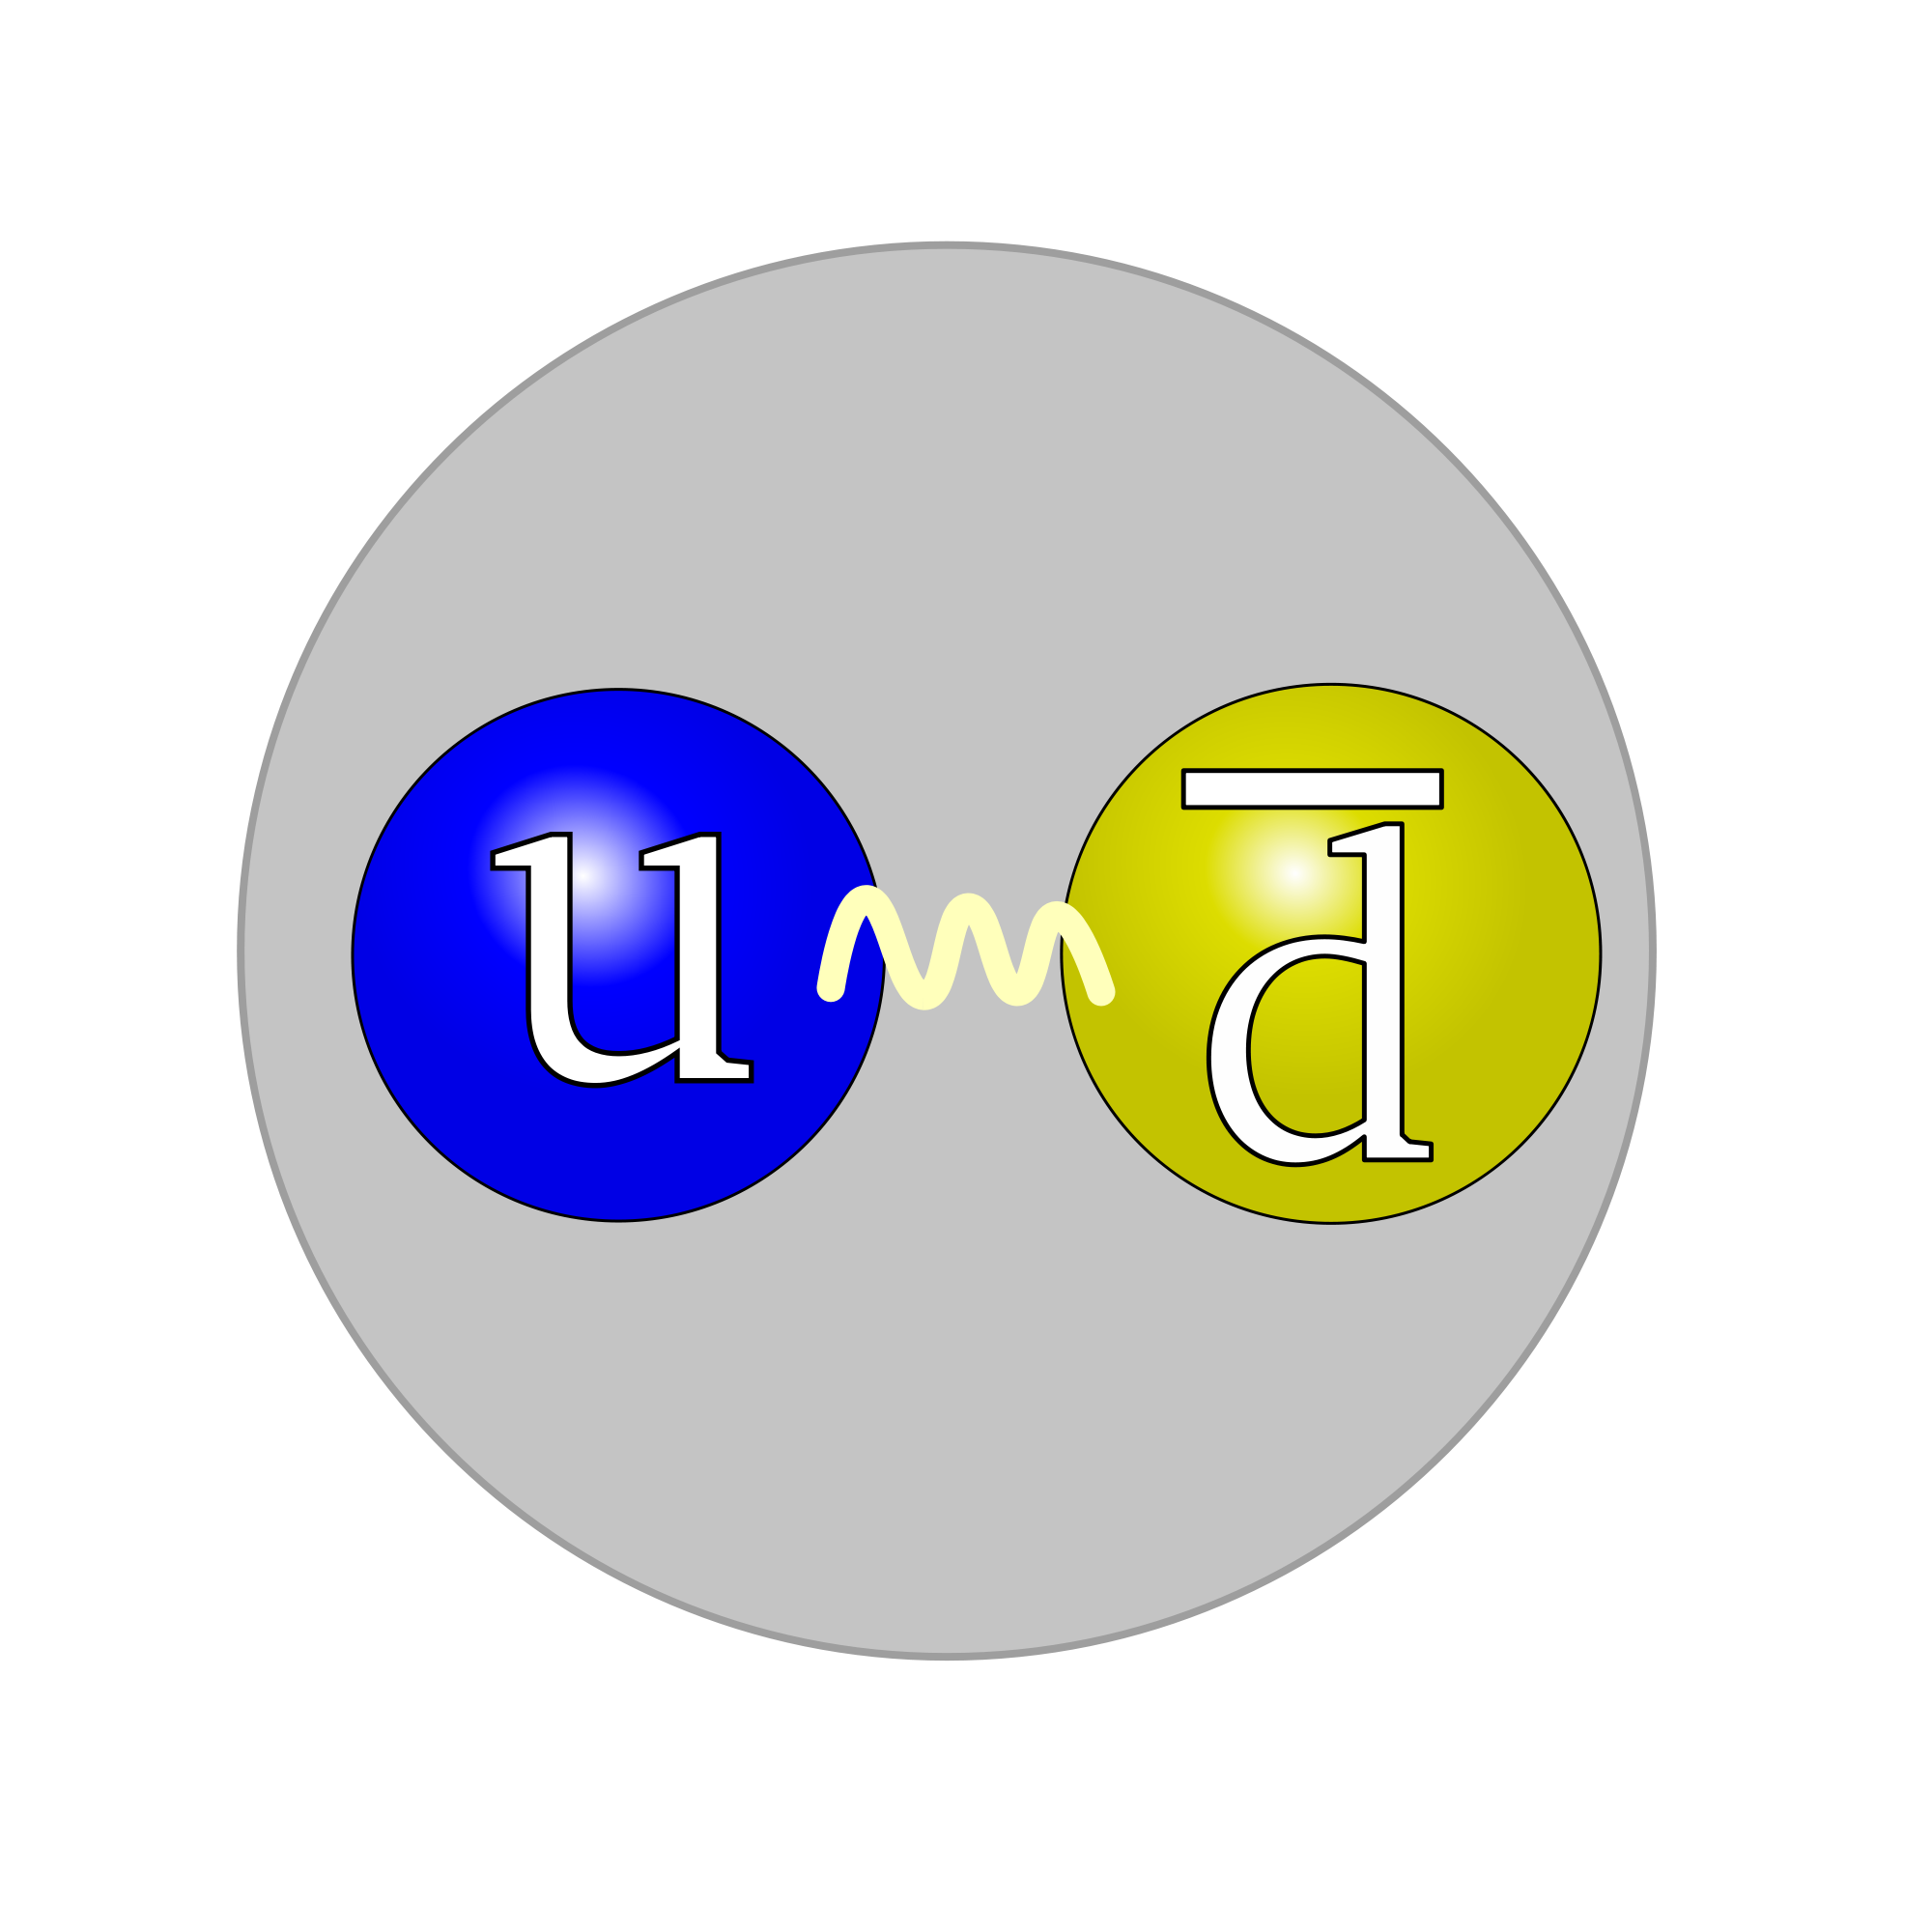
\includegraphics[width=0.5\textwidth]{ImgChap1/Meson2}
	\caption{Side view of the delta wing connector of the hodoscope}
	\label{DeltaWingSide}
\end{figure}

\begin{figure}[!ht]
	\centering
	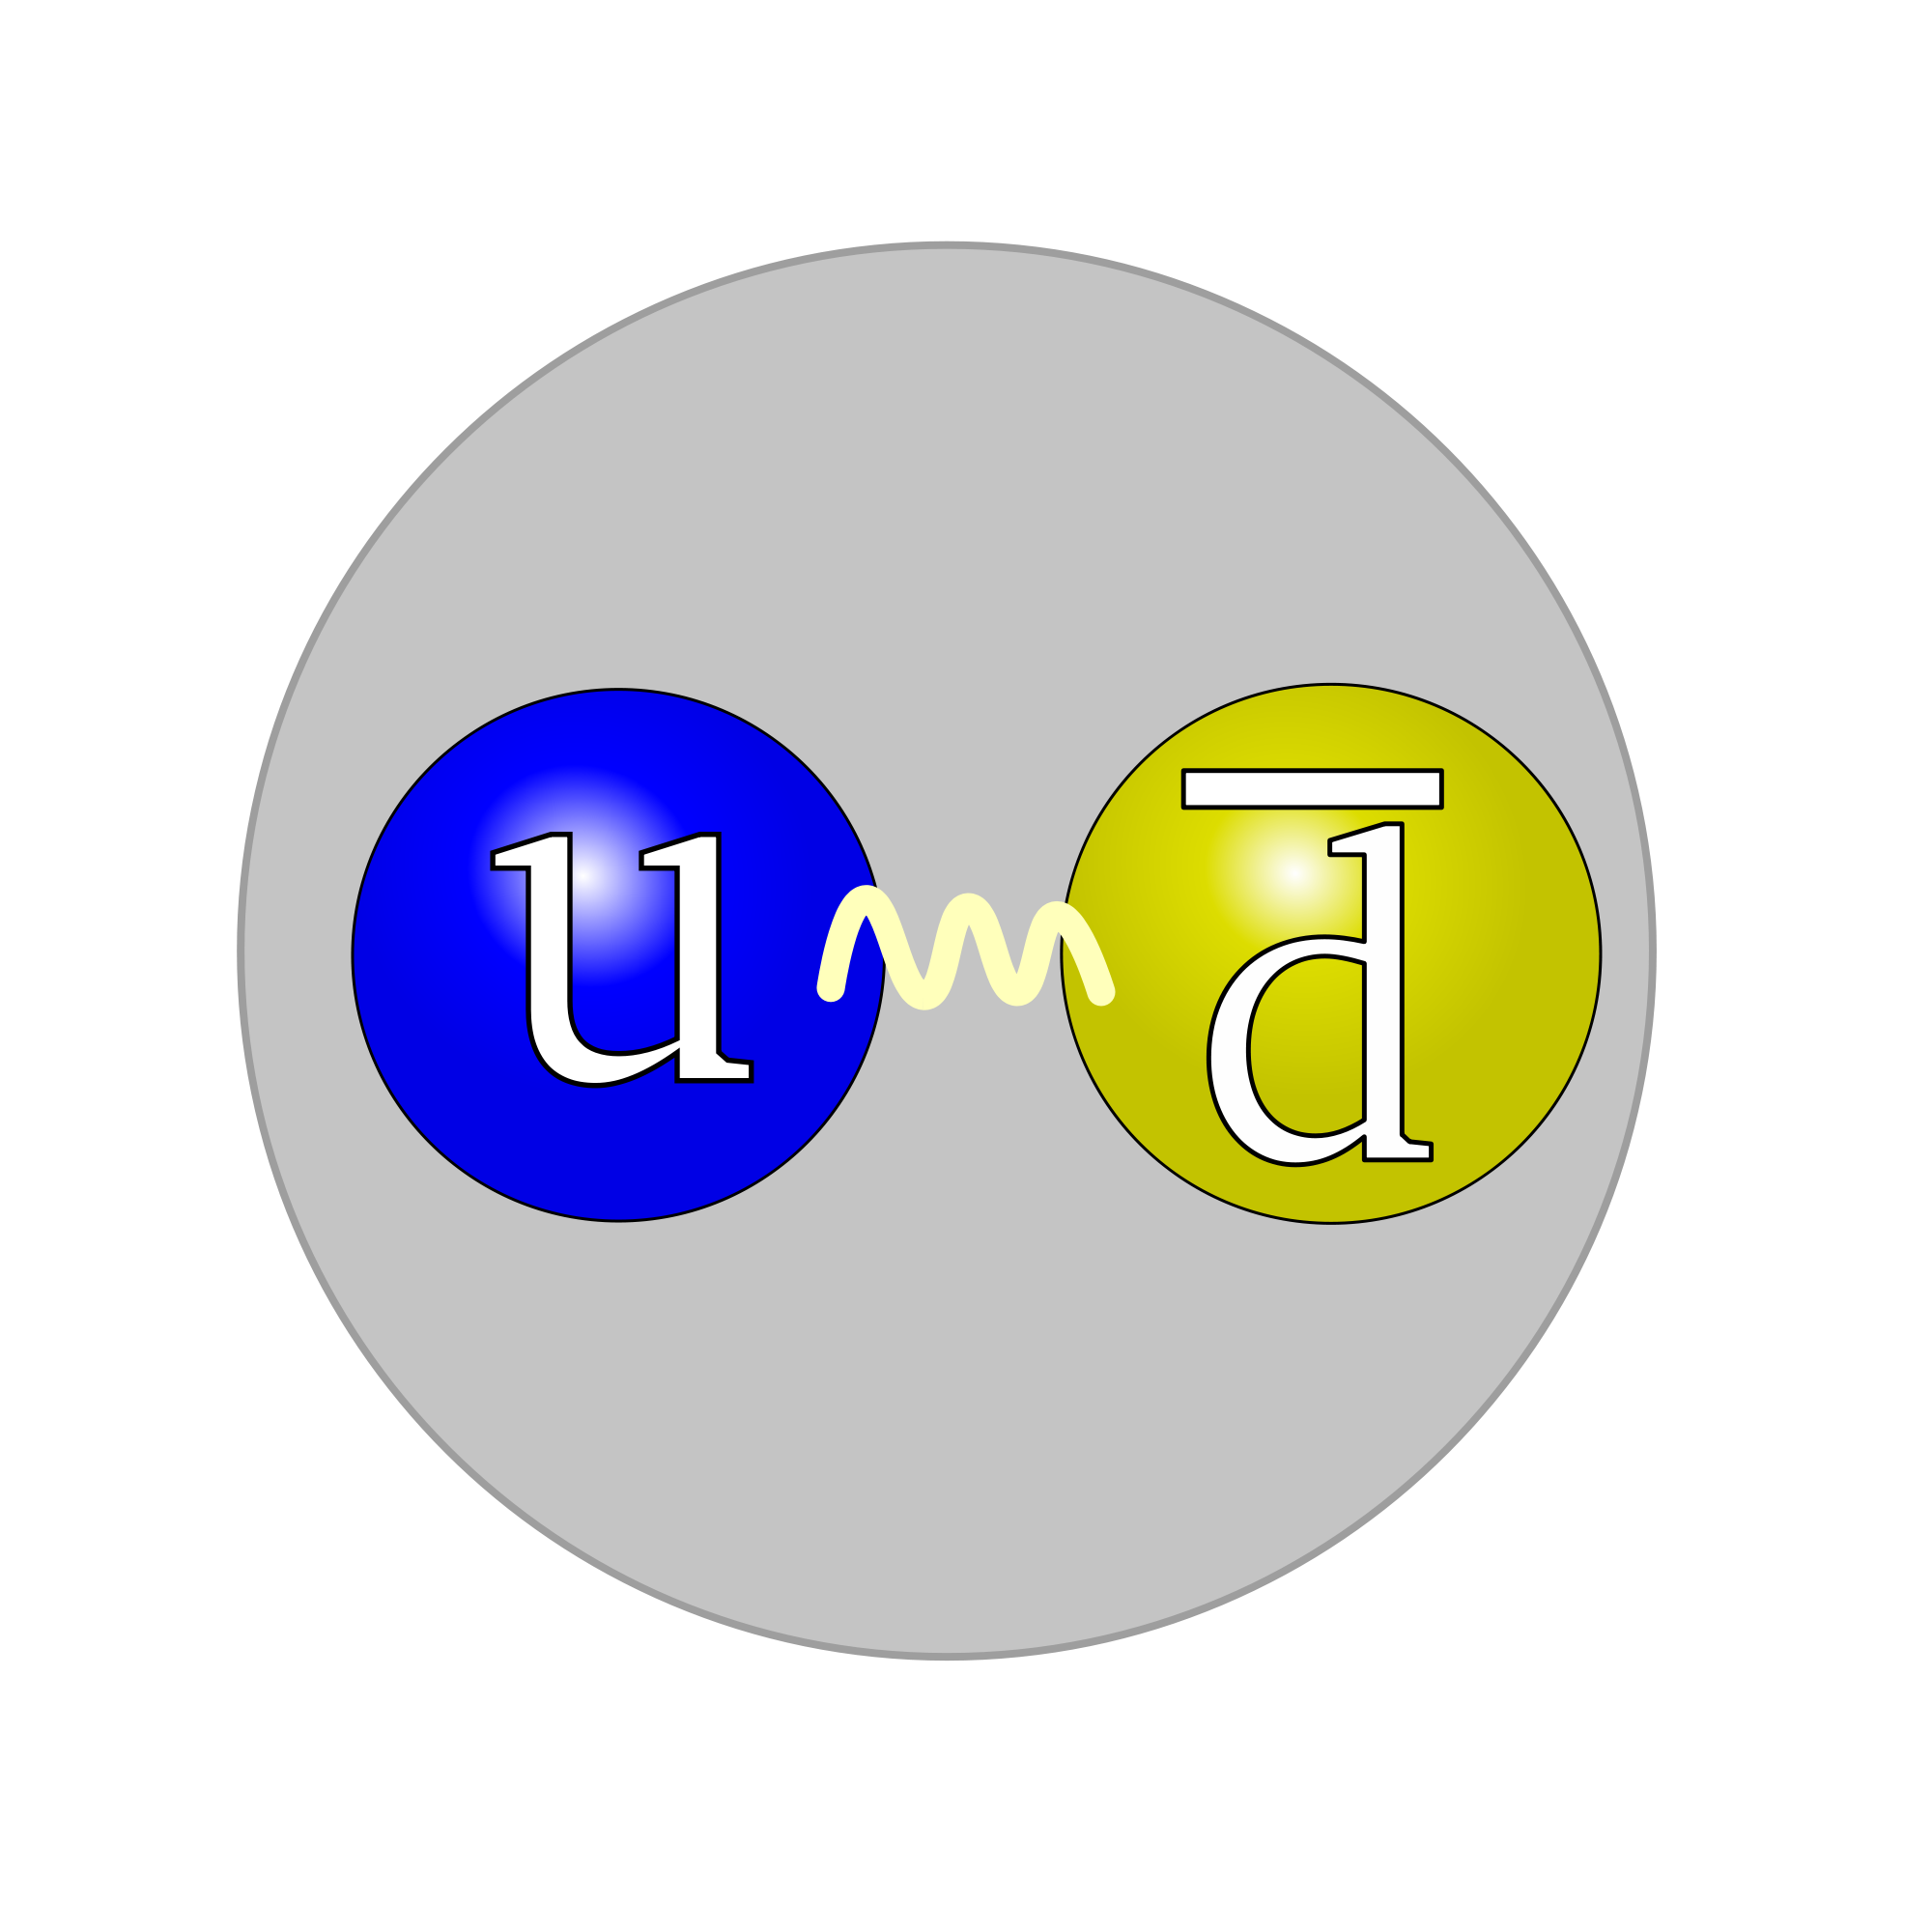
\includegraphics[width=0.5\textwidth]{ImgChap1/Meson2}
	\caption{Top down view of the delta wing connector of the hodoscope}
	\label{DeltaWingTop}
\end{figure}



\subsubsection*{Fishtale Fibre - SiPM connector}

The fishtale connections create a sealed juncture between the optical fibres and the Silicon photomultipliers. They act to guide the fibres precisely into position and maintain their optical isolation from the external environment. The connectors are 3d printed to create a consistent precise design to interface to all 30 groups of SiPMs. The fishtale connector is composed of 3 components, the main body comprising most of the length of the connector which takes in the appropriate fibres seperating from the main transport bundle of the detector. An interlocking end piece which interfaces with the electronics board and into which the fibre optic cables are glued. Finally a lipped lid which seals the construction from outside sources of noise. The fibres entry the main body through a flaired opening, which narrow to a channel just wide enough for 8 3.6mm sheaths to fit through, before curving wider, following a similar contour to a wine bottle. The flair entrance enables a wider angle of acceptance of fibre bundles. The narrow opening helps to minimise any light leaks into the component. The widening body allows the fibres to evenly spread out and be guided towards their respective SiPMs with a wide radius of curvature, minimising any loss of light and stress on the fibres. The fibre bundles pass through the main body still incased in their protective casing up until their juncture with a recess into the end piece of the connector, maintaining the isolation of fibre optics. 

\begin{figure}[!ht]
	\centering
	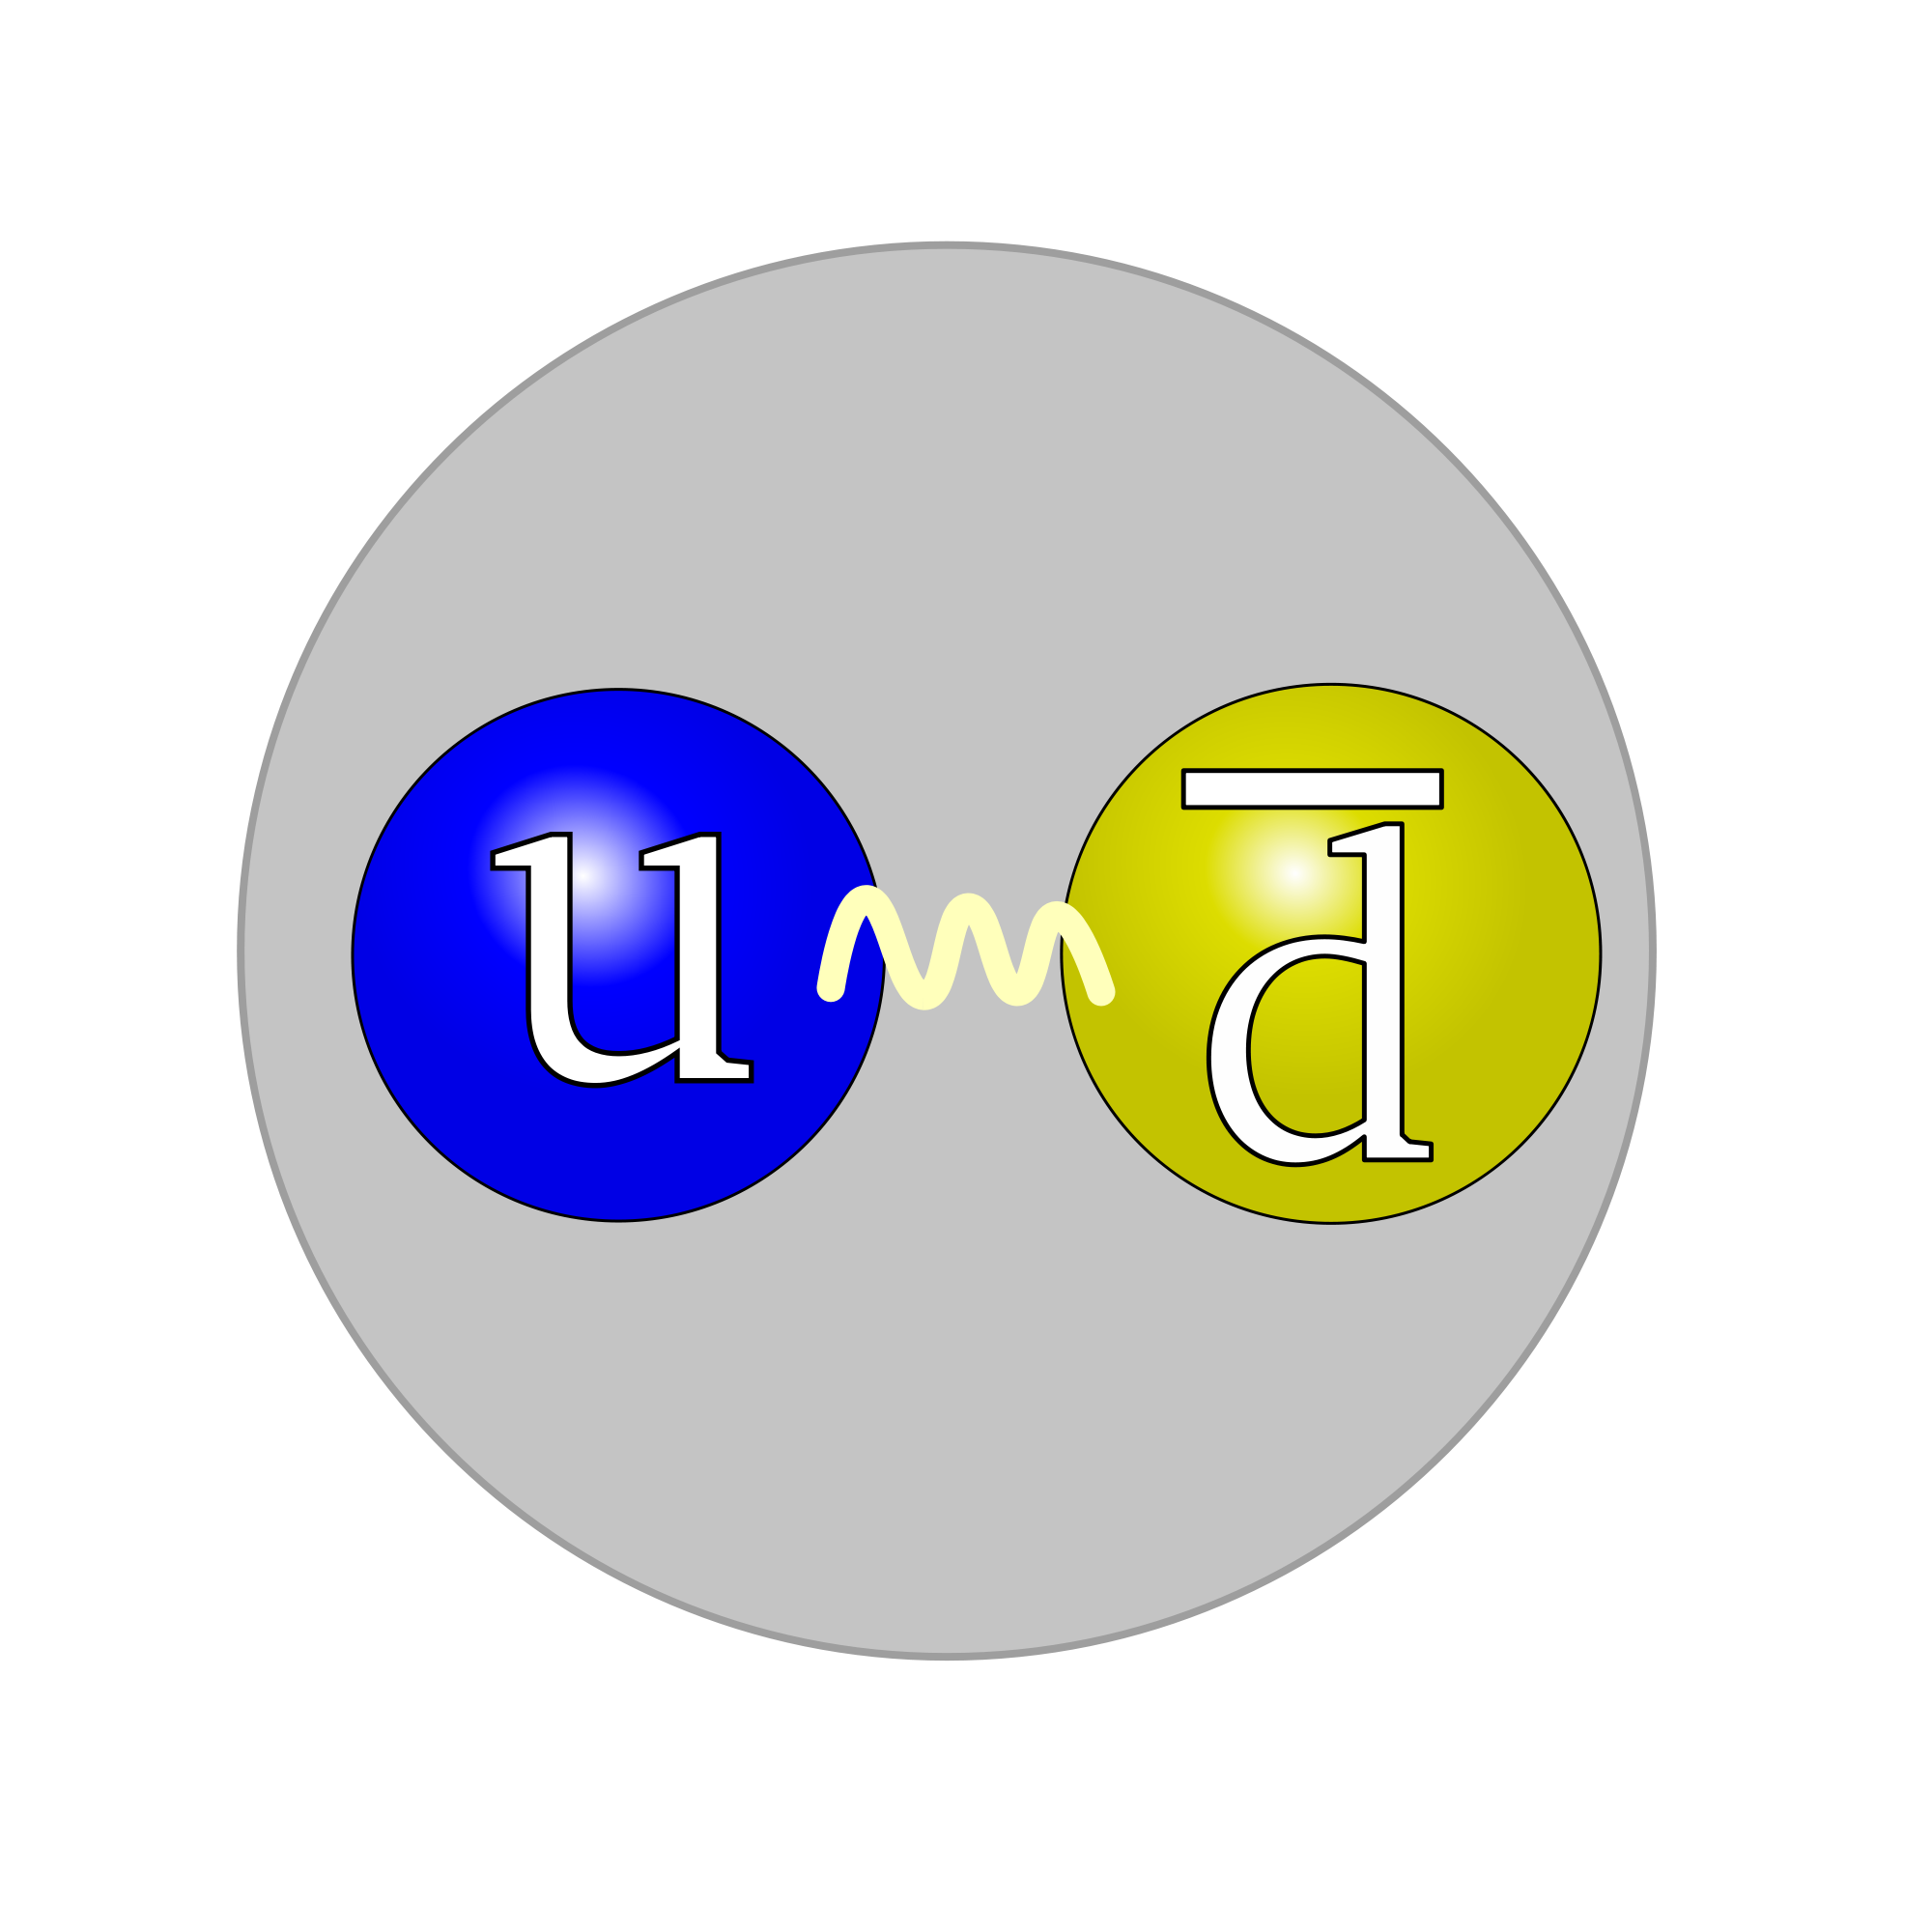
\includegraphics[width=0.5\textwidth]{ImgChap1/Meson2}
	\caption{Fishtale connector image}
	\label{FishtaleComplete}
\end{figure}

\begin{figure}[!ht]
	\centering
	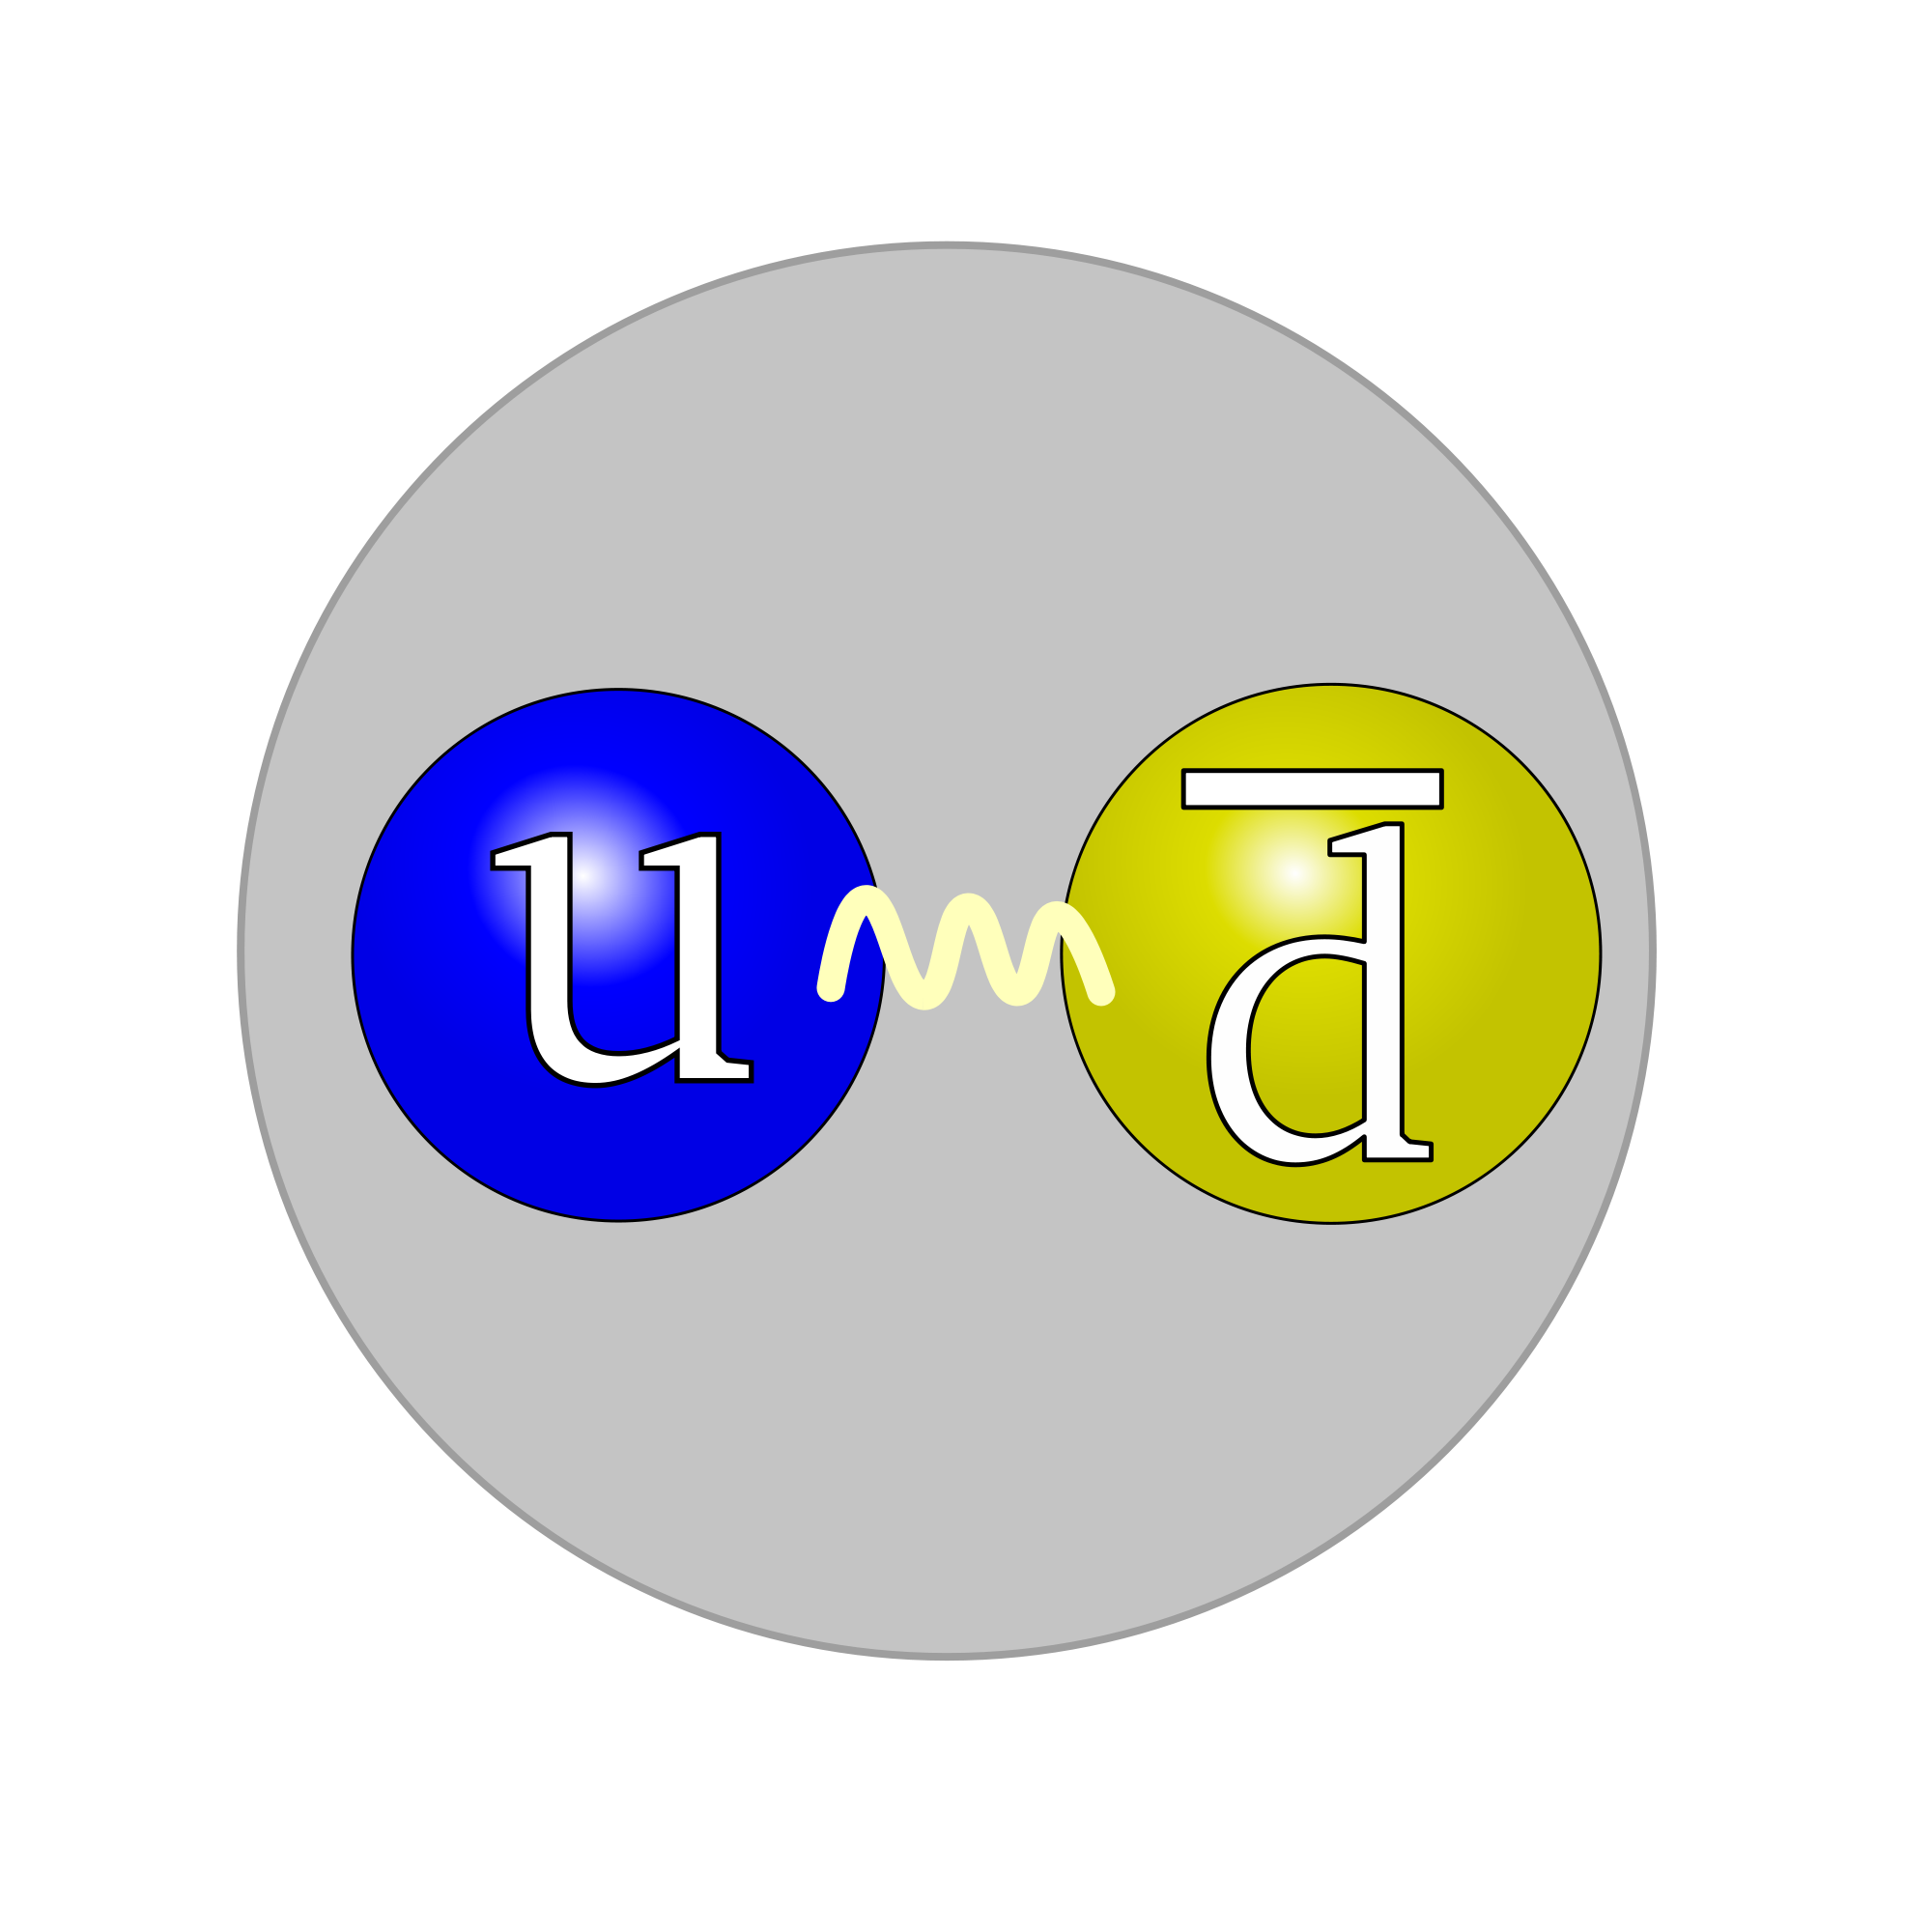
\includegraphics[width=0.5\textwidth]{ImgChap1/Meson2}
	\caption{Deconstructed fishtale connector image showing the different components of the fishtale connector}
	\label{FishtaleDeconstructed}
\end{figure}

It's critical that the optical connections formed between the connectors and the SiPMs are consistent between channels to maintain the calibration of the detector system.

\subsubsection*{Electronics Enclosure}

Carbon fibre plates
Band around the edge of the detector.
3d printed components
delta wing.
fishtail connectors
connector blocks with screws.
central ring fitting onto the tungsten pipe.
Support structure for the fibres passing through CLAS.
Electronics crate, light tight and cooled maybe.
Supastructure for construction, and transport.
etc.

\subsection{Lightsealing and protection}
How the different sections of the hodoscope are isolated from any outside sources of light and also crosstalk between elements, fibres and the electronics.


\subsection{Silicon Photomultipliers}

Silicon photomulitpliers (SiPM) are a very highly sensitive radiation detector with high efficiency and potential for very precise timing resolution. They are designed to trigger on single photons of light with high efficiency producing a signal with high gain and very low time jitter of <100ps. They are designed to be highly segmented allowing many photons to be detected simultaneously, with each element isolated from one another to avoid unnecessary background noise producing highly precise clean signals.

SiPMs consist of a matrix of highly sensitive micro cell (pixels) all connected in parallel. Each one is composed of a Geiger-Mode avalanche photon diode (GM-APD)with a connected to a resistor for passive quenching, Figure \ref{SiPMCircuit}. When operating above a certain breakdown voltage the diode rapidly discharges once triggered by a photon or another source of noise producing a signal with a high gain, before the resistor acts to quench the discharge and the cell will switch to a recovery mode where the capacitor in the diode is recharged ready to trigger again. 

\begin{figure}[!ht]
	\centering
	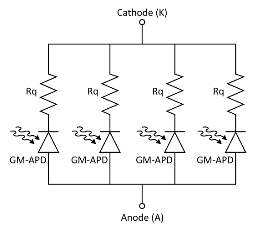
\includegraphics[width=0.5\textwidth]{ImgChap1/SiPM1}
	\caption{A schematic representation of the parallel arrangement of Geiger-Mode avalanche photo diodes with quenching resistors in a silicon photomultiplier. \cite{website:AdvanSiDSiPMpdf}}
	\label{SiPMCircuit}
\end{figure}

\begin{figure}[!ht]
	\centering
	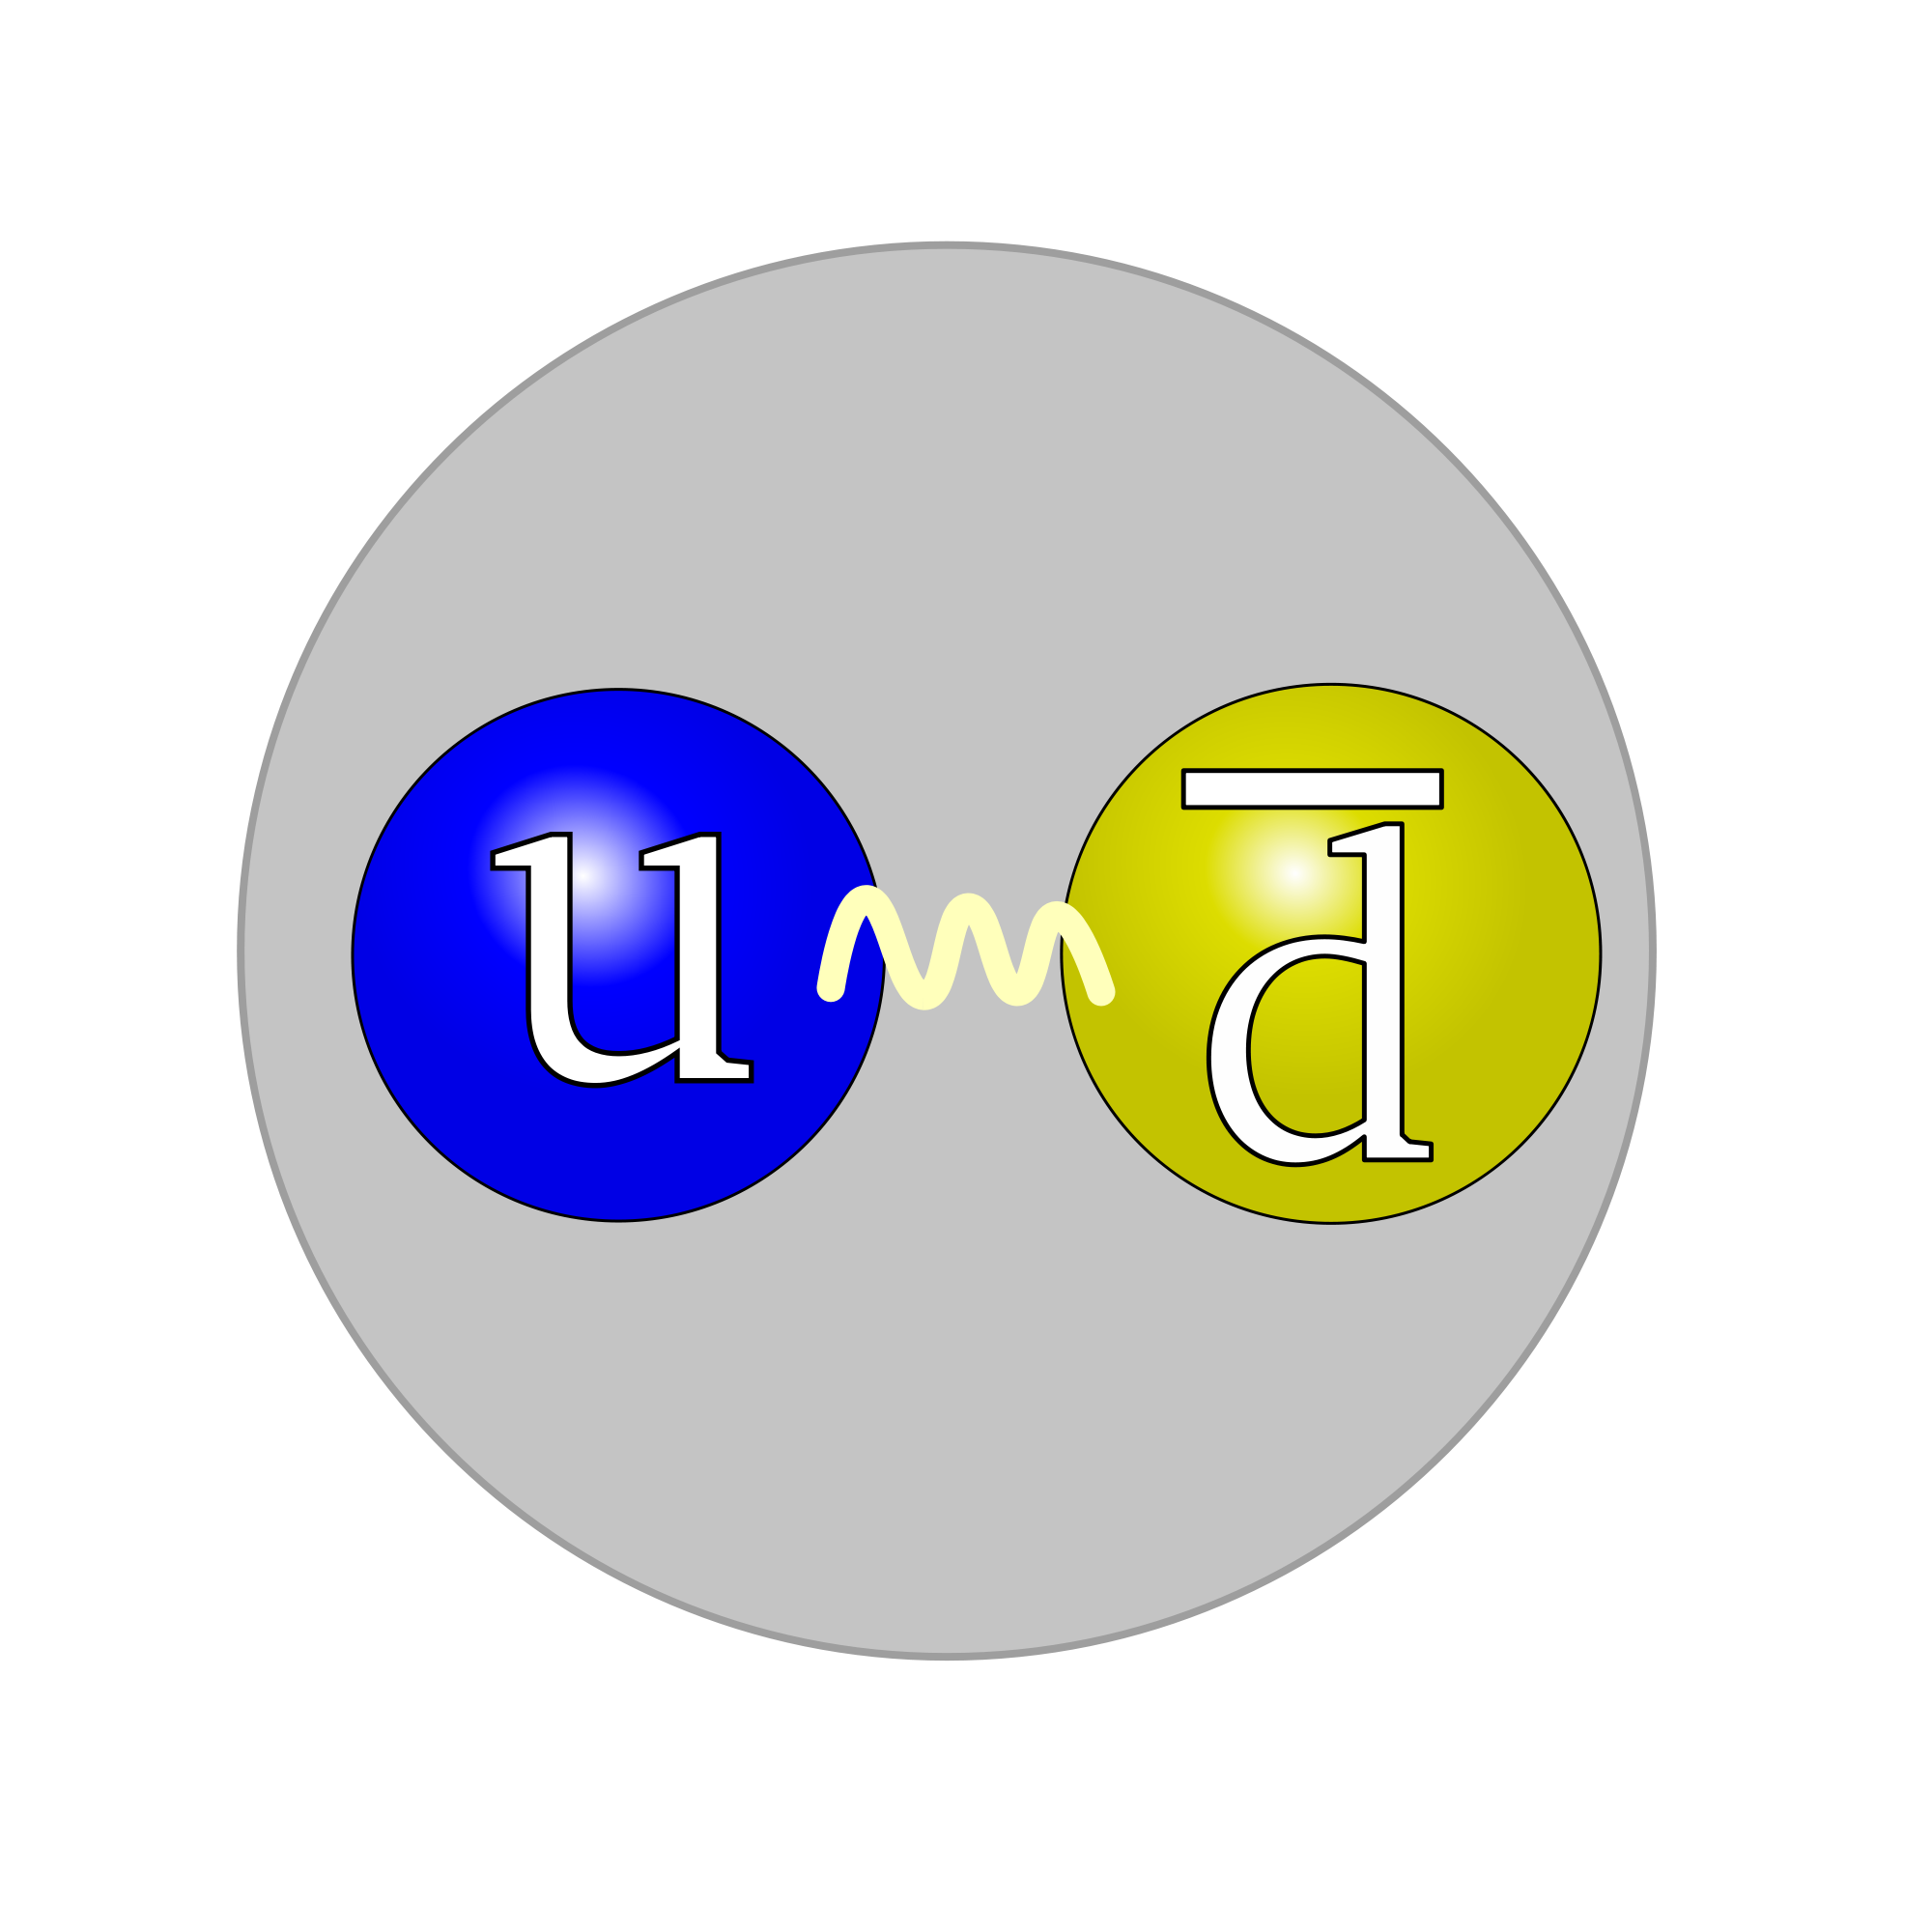
\includegraphics[width=0.5\textwidth]{ImgChap1/Meson2}
	\caption{Picture of a typical SiPM signal showing the rapid discharge phase followed by the slower recharge phase.}
	\label{SiPMDischargeRecharge}
\end{figure}

\subsubsection*{Photon Detection Efficiency}

The probability of a pixel triggering on the arrival of a incoming photon to the SiPM is known as the photon detection efficiency (PDE). This is defined as a product of three factors, quantum efficiency, triggering probability and geometry efficiency: 

\[ PDE(OV) = Qe \times Pt(OV) \times Ge \]

Quantum efficiency (Qe) expresses the probability that a photon transitions into and is absorbed by the silicon and is converted in an electron/hole pair. Qe is a function of the photons wavelength and and angle of incidence upon the SiPM. This factor is the critical reason for the wavelength shifting fibres used in the hodoscope. Triggering probability (Pt) is the likelihood that an electron/hole pair successfully triggers a sustained avalanche process resulting in a current pulse. This value is highly dependent on the overvoltage, above breakdown, applied to the circuit. Rising rapidly with increasing voltage. Pt is also wavelength dependent as the probability of generating an avalanche depends on the creation position of the electron/hole pair, which is dependent on the wavelength of the incident photon. The geometry efficiency also known as the fill factor, is a function of the amount of dead area present on the surface of the SiPM. This is a necessity to accommodate structures to isolate the pixels from one another, however with improved designs and advancing techniques for silicon lithography, the active area of the device can be optimised.

\subsubsection*{Sources of Noise}

The primary source of noise in SiPMs is the dark count rate which appear as uncorrelated pulses in the absence of light. These are a result of electron/hole pairs created by thermal excitations in the active region of a GM-APD, mimicking the appearance of a genuine single photo electron trigger pulse. The dark count rate (DCR) for a SiPM is dependent on temperature, approximately doubling every 10$^{\circ}$C. It scales directly with the area of the device and is an increasing function of the overvoltage applied to it. During operation the DCR for the hodoscope will be close to 1Mhz, however because the pulses are uncorrelated, have short rise and fall times and their amplitudes are tiny compared to a signal pulse, the dark events can be filtered with a simple discriminator at the level of 1.5 photo electrons. \cite{website:AdvanSiDSiPMpdf}

In addition to the primary noise, there are two sources of correlated noise in SiPMs. Afterpulsing (AP) and optical crosstalk (OC). Both of these types of events originate from an existing current event (Either a photon event or a dark event) and are largely dependent on the current density of the original event and the trigger probability Pt. Afterpulsing results from charge carriers trapped in silicon defects during discharge that are released later during the recharge phase of a cell. This results in a new current pulse produced on the tail of the true event, typically a few ns after the original peak. Optical crosstalk involved photons that are produced during an avalanche leaking into the active area of a neighbouring cell triggering another avalanche, known as direct OC, or is re-absorbed into an inactive region of a cell. Those in the inactive region can then diffuse back into the active region of the cell causing another pulse with a short time delay (the order of a few ns) with respect to the original signal. Both AP and OC increase more than linearly with overvoltage and quadratically with cell size, for more details see \cite{gola2012sipm}.


\subsubsection*{Operation in the hodoscope}

SiPMs high efficiency, high gain, fast timing responce and ability to trigger on single photons make them ideal for a fast timing scintillating detector such as the FT-Hodoscope. They are used in place of standard photomultiplier tubes as the detection mechanism for the photons produced in each scinillator tile. Each tile is read out by a 3x3mm array of Hamamatsu SiPMs with a pixel pitch of 75 $\mu m$ and a fill factor of 82$\%$ this provides 1600 pixels for a maximum expected signal size of 200 photons. Each tile is connected to the SiPMs by fibres, which shift the wavelength of the photons into the ideal range to maximise the quantum efficiency of the SiPMs. The gain of the detectors is very sensitive to the voltage applied, they require a supply stable to within 0.01V to maintain a consistent response level. The operating voltage for each SiPM is individually calibrated and adjusted using variable resistors assigned to each channel. 

Another consideration is the operating temperature of the SiPMs, as this affects both the dark count rate and the gain of the channels. Keeping the temperature at the lower end of the operating range keeps the dark noise to a minimum and it needs to be stable to properly calibrate the gain of the detector. At lower temperatures, that suppress the level of dark noise in the detector, higher overvoltages can be applied to the system, increasing the probability that a photon generated electron/hole pair will trigger an avalanche, increasing the photon detection efficiency of the SiPM. A typical signal from a minimum ionizing particle interacting with a detector element in the hodoscope, will result a signal with a magnitude of between 40 and 100 photoelectrons. This is far larger than the levels of signals produced through dark noise, typically 1-3 photoelectrons when crosstalk is included. As a result the signal peaks can be easily seperated from the dark noise from a simple discriminator cut at the 5-10 photoelectron level without signal loss. As a result, although desirable to maintain operation at a lower temperature, the main consideration for the hodoscope is temperature stability during operation. While in operation in hall B the detector will be maintained at a nearly constant temperature by the atmosphere control systems in the hall.

When a large number of photons arrive at the detector, several parallel cells can trigger simultaneously, the amplitude and area of the pulse generated is proportional to the number of cells that fired. This allows both the integral of the pulse and the pulse height to be used to determine the amount of photoelectrons generated in the SiPMs. A signal of around 10 photoelectrons in magnitude would be enough to have confidence that a pulse is a signal not generated through thermal excitations. However, simulations indicate that producing a signal of 40+ photoelectrons is required to produce the <500 ps timing resolution the detector is designed to surpass.





Short Paragraph about how they fundamentally work, how they recover and when they are ready for operation again. Cover breakdown voltage etc. Can talk about how this is affected by temperature here maybe?

Photon detection efficiency, what affects this etc? 

Noise sources.

How they fit into the operation of the hodoscope.

High frequency dark current.
High gain for small signal.
High signal to noise ratio when triggered.
Very sensitive to light leaks.
Very sensitive to voltage range. Requires a relatively low high voltage at around 70V. But ideally requires a HV sensitve to 0.01 V. for effective calibration.
Sensitive to temperature range.
Do not work up to a certain voltage then rise in gain quickly beyond this.
Noise peaks can be used for calibration.
Different pixel sizes. A single pixel can only fire once for each photon arriving in an event. Need enough pixels so some are not lost to double hits.
Photon conversion efficiency, Probability for a photon arriving to cause an avalanche. Function of available live area, voltage and SiPM type. Newer versions greatly improved these properties.
Output from the detector needs to be spread accross the surface of the SiPM to maximise light trigger efficiency.
3x3 arrays of sensors used for this detector system. $75\mu$m pixels. Ammount of dead area reducing with new generations.
Reduction in cross talk between pixels. Multi pixel noise mostly due to cross talk between nearby pixels causing near simulataneous firing.
Works in strong magnetic fields, not necessary in this experiment but may be of relevance in the future. Normal PMTs cannot work in that environment.
Tiny size allows them to be packed very densely allowing possibilities for extremely finely segmented detectors with individual read-out for each channel.

Fundementals, how to they work? Limited information on the electronics as this is not an area of expertise.
Focus more on their strengths and weaknesses and applications to physics.
Discuss quantum efficiency, trigger probability and fill factor combining to produce the photon detection efficiency.
Discuss gain and the factors that influence it.
Discuss noise, both primary (dark noise) and correlated (afterpulsing, crosstalk etc.)

\cite{barbosa2012silicon}
\cite{degtiarenko2011calculation}
\cite{lightfoot2008characterisation}
\cite{website:AdvanSiDSiPMpdf}

\subsection{Electronics}
Mezzanine and pre amp boards were developed and designed in Genoa with some feedback from our testing. Designed to work with the silicon photo multipliers. Levels of gain are critical to allow for the full dynamic range of signals to be captured. The extremely low levels of noise compared to the signal amplitude allow very high signal to noise ratio to be achieved with a low threshold discriminator.
Control boards. Adjusting the voltage and monitoring the temperature for each channel.
High and low voltage units, stability and precision voltage levels are critical.
Flash ADCs.

\subsection{Reflective materials}

High performance reflective materials are critical for optimising the optical properties of the detector. The material used to surround the scintillating tile elements requires the following properties:
\begin{itemize}
	\item High co-efficient of reflectivity  
	\item Consistent performance across tiles
	\item Minimal thickness
	\item Radiation Hard
\end{itemize}

These qualities are required to maximise the light collection of the wavelength shifting fibres improving the timing resolution of the detector. To provide consistent performance across individual elements and also over the lifetime of the detector. Finally to optically isolate each element ensuring there is no potential for crosstalk and minimising the affect of any light leaks into the system.

A high co-efficient of reflectivity is critical to keep photons produced through scintillation inside the detector elements and provide additional opportunities for photons that aren't quickly captured by the wavelength shifting fibres to reflect off the surfaces and be collected by the fibres. The co-efficient of reflectivity for a material is a function of the wavelength of light that it encounters. In this case the critical range is the emission spectrum of EJ-204, Figure , which ranges between 380nm and 500nm, peaking at around ~410nm. The higher the co-efficient of the material across the active range of the material, the higher than potential light yield from the tile.


\begin{figure}[!ht]
	\centering
	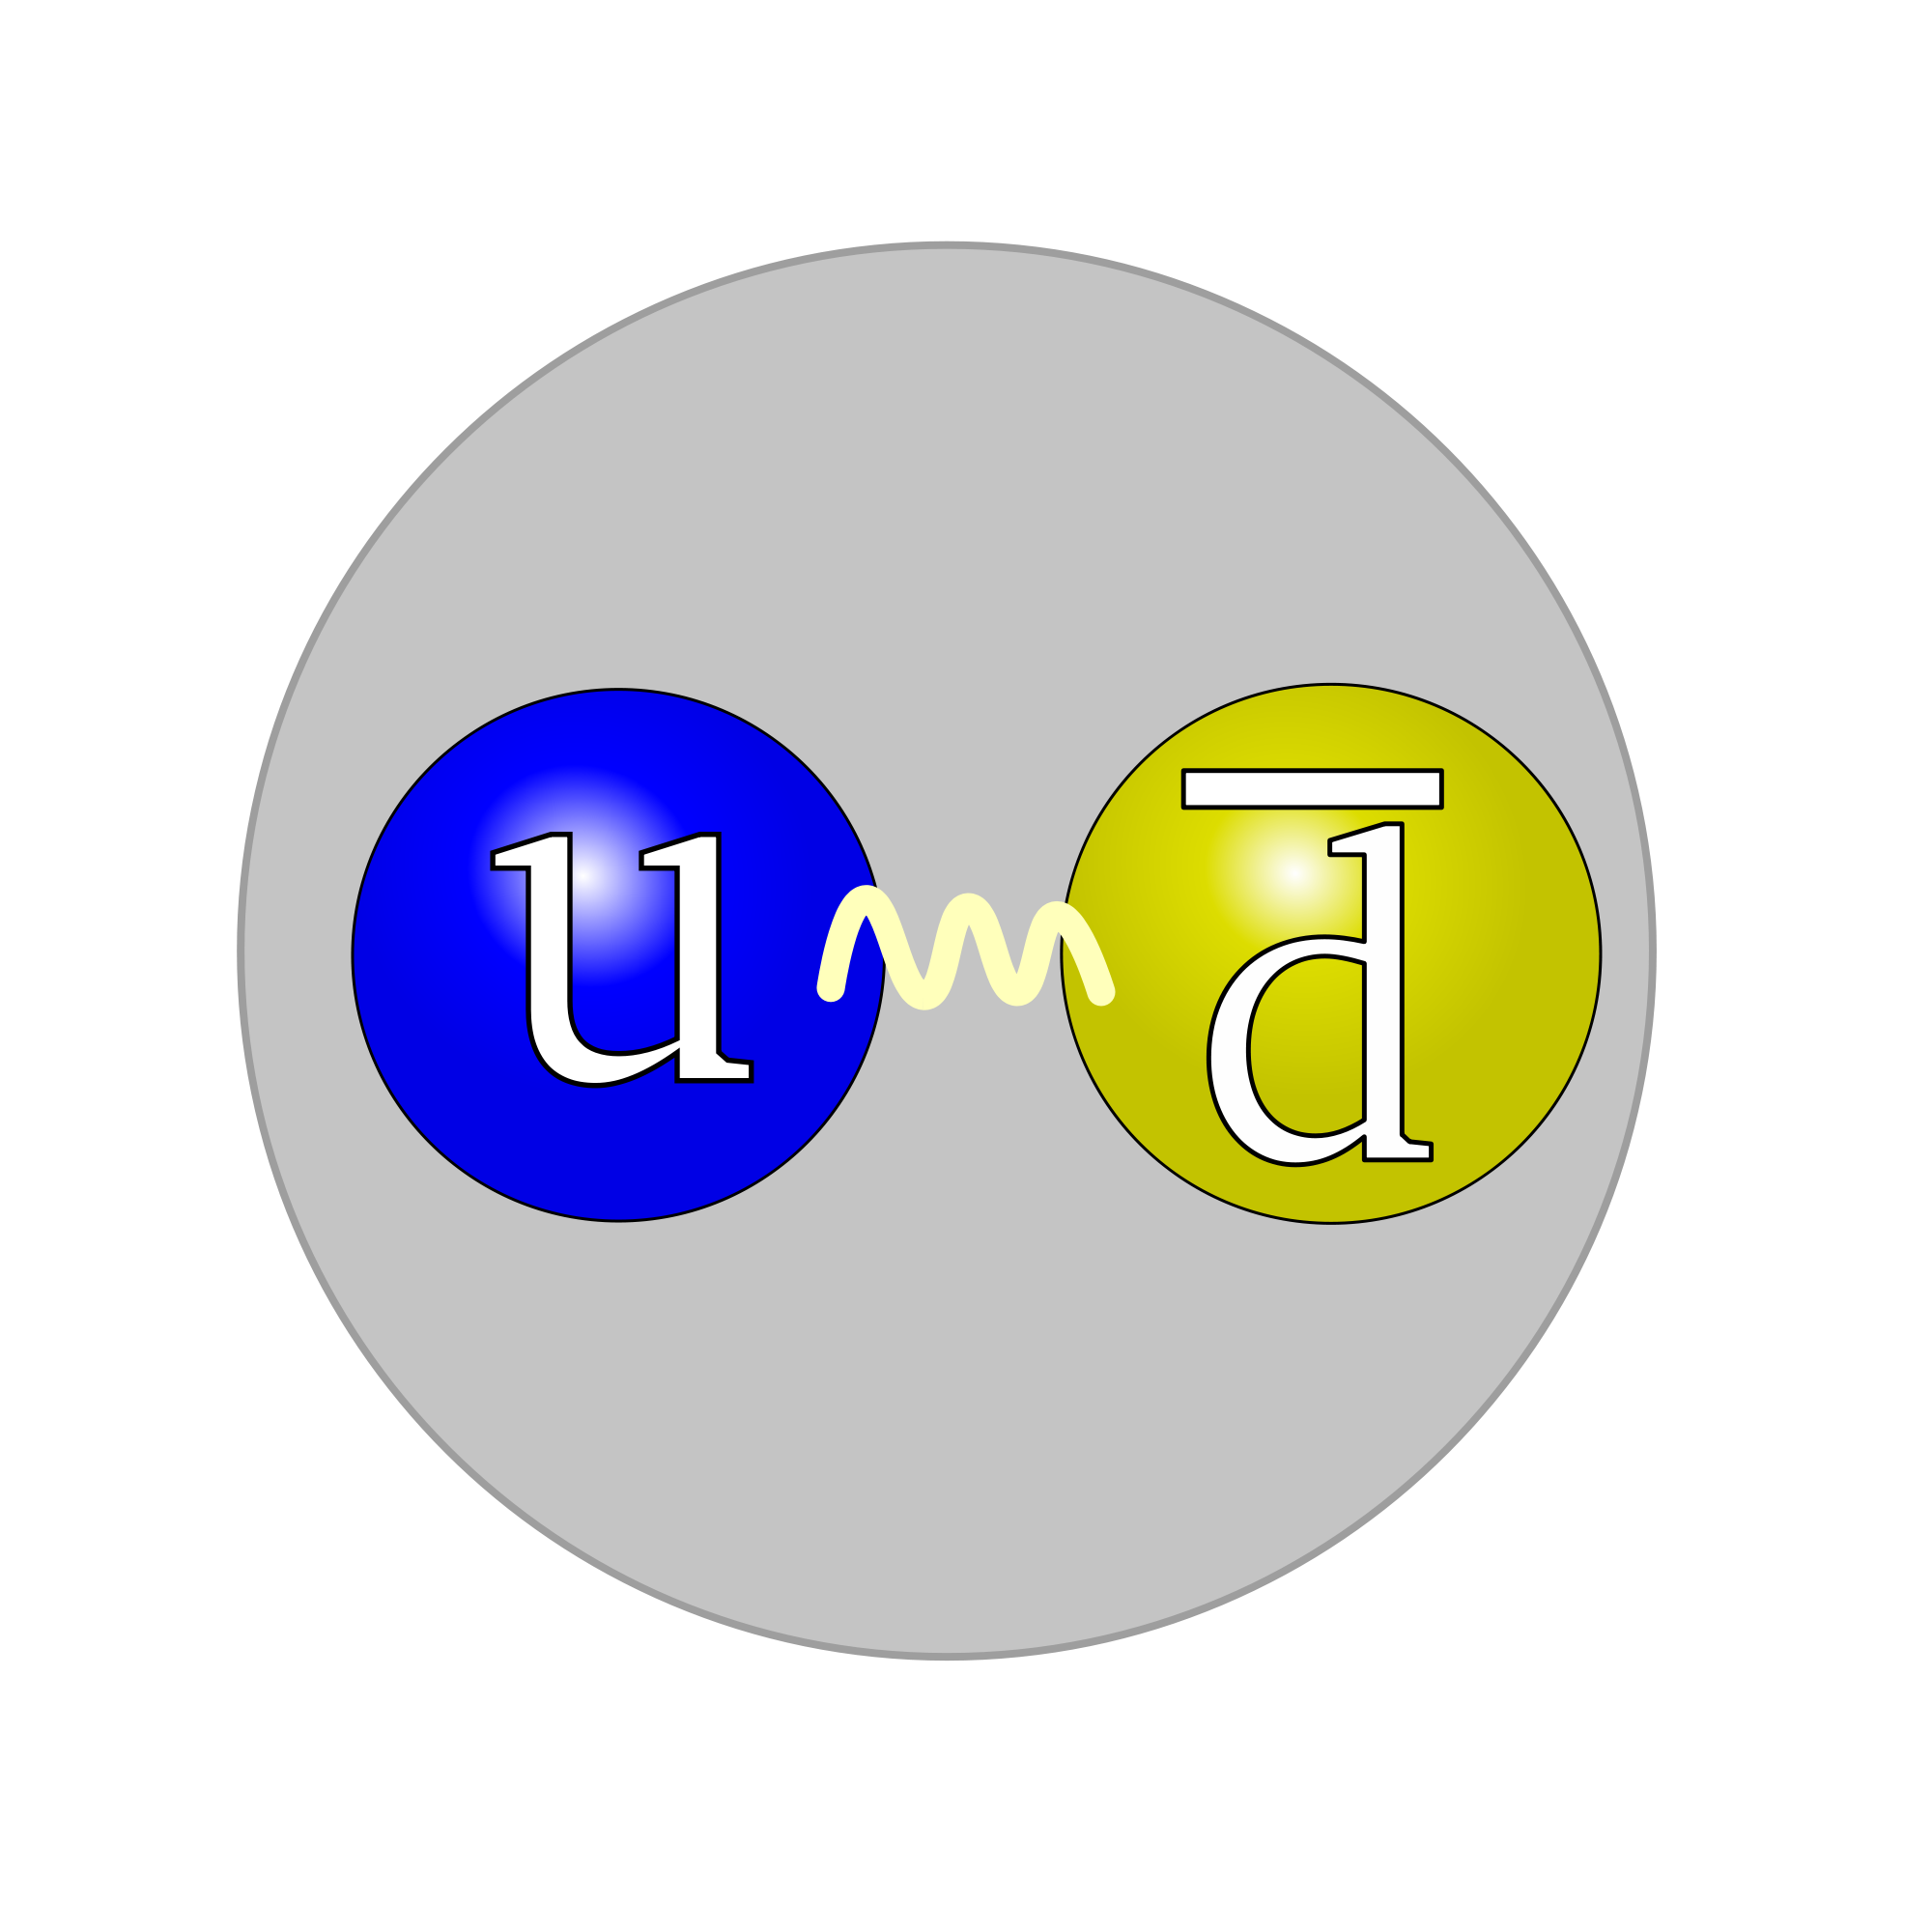
\includegraphics[width=0.5\textwidth]{ImgChap1/Meson2}
	\caption{Reflection coefficient for several reflectors as a function of wavelength.  \cite{janecek2012reflectivity}}
	\label{ReflCoef}
\end{figure}

Consistency of response to a incoming charge particle is very important in a highly segmented detector such as the hodoscope, if results from different elements are to be interpreted together. The reflective material itself must be consistent in both its response to photons but also in its juncture to the detector elements. It must be able to be moulded with precision to the shape of the detector blocks without uneven surfaces or air gaps and maintain its shape over the lifetime of the detector under the harsh radiation of the beamline. A material which may theoretically be superior in an idealised situation. May not perform or have inconsistent results when applied over many different elements. As a result systematic testing is required to ensure any materials forfill the design requirement and ease of application becomes a more significant factor than one may a priori consider.

One of the typical disadvantages of segmented detectors is a reduction in the active area of acceptance with any gaps between elements. To keep this reduction to a minimum the tiles need to be of a uniform size that will tessellate with minimal area covered by non active materials such as a reflective material. Therefore the ideal reflector is formed of a vanishingly thin layer of the material, however the reflectivity of a material is also dependent on its thickness, with multiple layers improving the co-efficient of reflectivity. In addition with minimal thickness comes fragility and often inconsistency. A balance between these factors is required.

During operation the detector and its reflective elements will be subjected to significant levels of radiation, with a typical flux of \textbf{PLACEHOLDER} krads. The reflective materials need to maintain their performance above design requirements without significant degradation over the lifetime of the detector. Replacement of the material during its lifetime will not be possible without substituting the complete detector element and possibly causing further problems with nearby elements. Only materials known to be radiation hard under these conditions were considered for use in the detector.  

Considering only materials that fulfilled the previously discussed criteria sample tiles were prepared with the reflectors shown in table \ref{ReflMatProp}. For each material tests were carried out using several samples of both p30 thin and p30 thick tiles, checking for consistency of results and any affects of the varying geometry. It also provided experience in the difficulty associated with preparing the tiles with each reflector. Considering that batch production would be required for the final system. To limit the possible variance of optical connections between the tile and the silicon photomultipliers, a simple air connection between the fibre and the tile was used which allowed the rest of the test configuration to be maintained constant for all tests. Tests were carried out using both Sr\textsuperscript{90} and Bi\textsuperscript{207} sources, both dominantly $\beta$ emitters with a range of peak energy commissions. Although data collected utilising cosmic rays would provide a more precise measure of photon output, tests conducted using sources can be completed much more quickly with statistically significant results. The trigger frequency for each tile-reflector configuration was measured for series of trigger values for a discriminator. \textbf{SEARCH OLD LAPTOP FOR FURTHER DATA ON THE RESULTS OF THESE TESTS}


	\begin{table}\centering
	\renewcommand{\arraystretch}{1.3}
	\begin{tabular}{ @{}l  c  c  c@{}} 
		\toprule
		Reflector & Reflection Coeficient & Thickness & Reference \\
		& {\small @440nm}& {\small [mm]}&  \\
		\midrule
		Titanium Dioxide Paint & 0.955 & 0.14-0.18 & \cite{janecek2012reflectivity}\\
		PTFE Tape & 0.99 & n x 0.08 &\cite{janecek2012reflectivity}\\
		Tyvek\textsuperscript{\textregistered} Paper & 0.97 & n x 0.11 & \cite{janecek2008optical} \\
		Aluminium Foil & 0.78 & 0.025 & \cite{janecek2008optical}\\
		\bottomrule
	\end{tabular}
	\caption{Properties of reflectors selected for testing}
	\label{ReflMatProp}
	\end{table}

\textbf{THE KEY RESULTS OF THE TESTS ARE SHOWN IN FIGURE}

\begin{figure}[!ht]
	\centering
	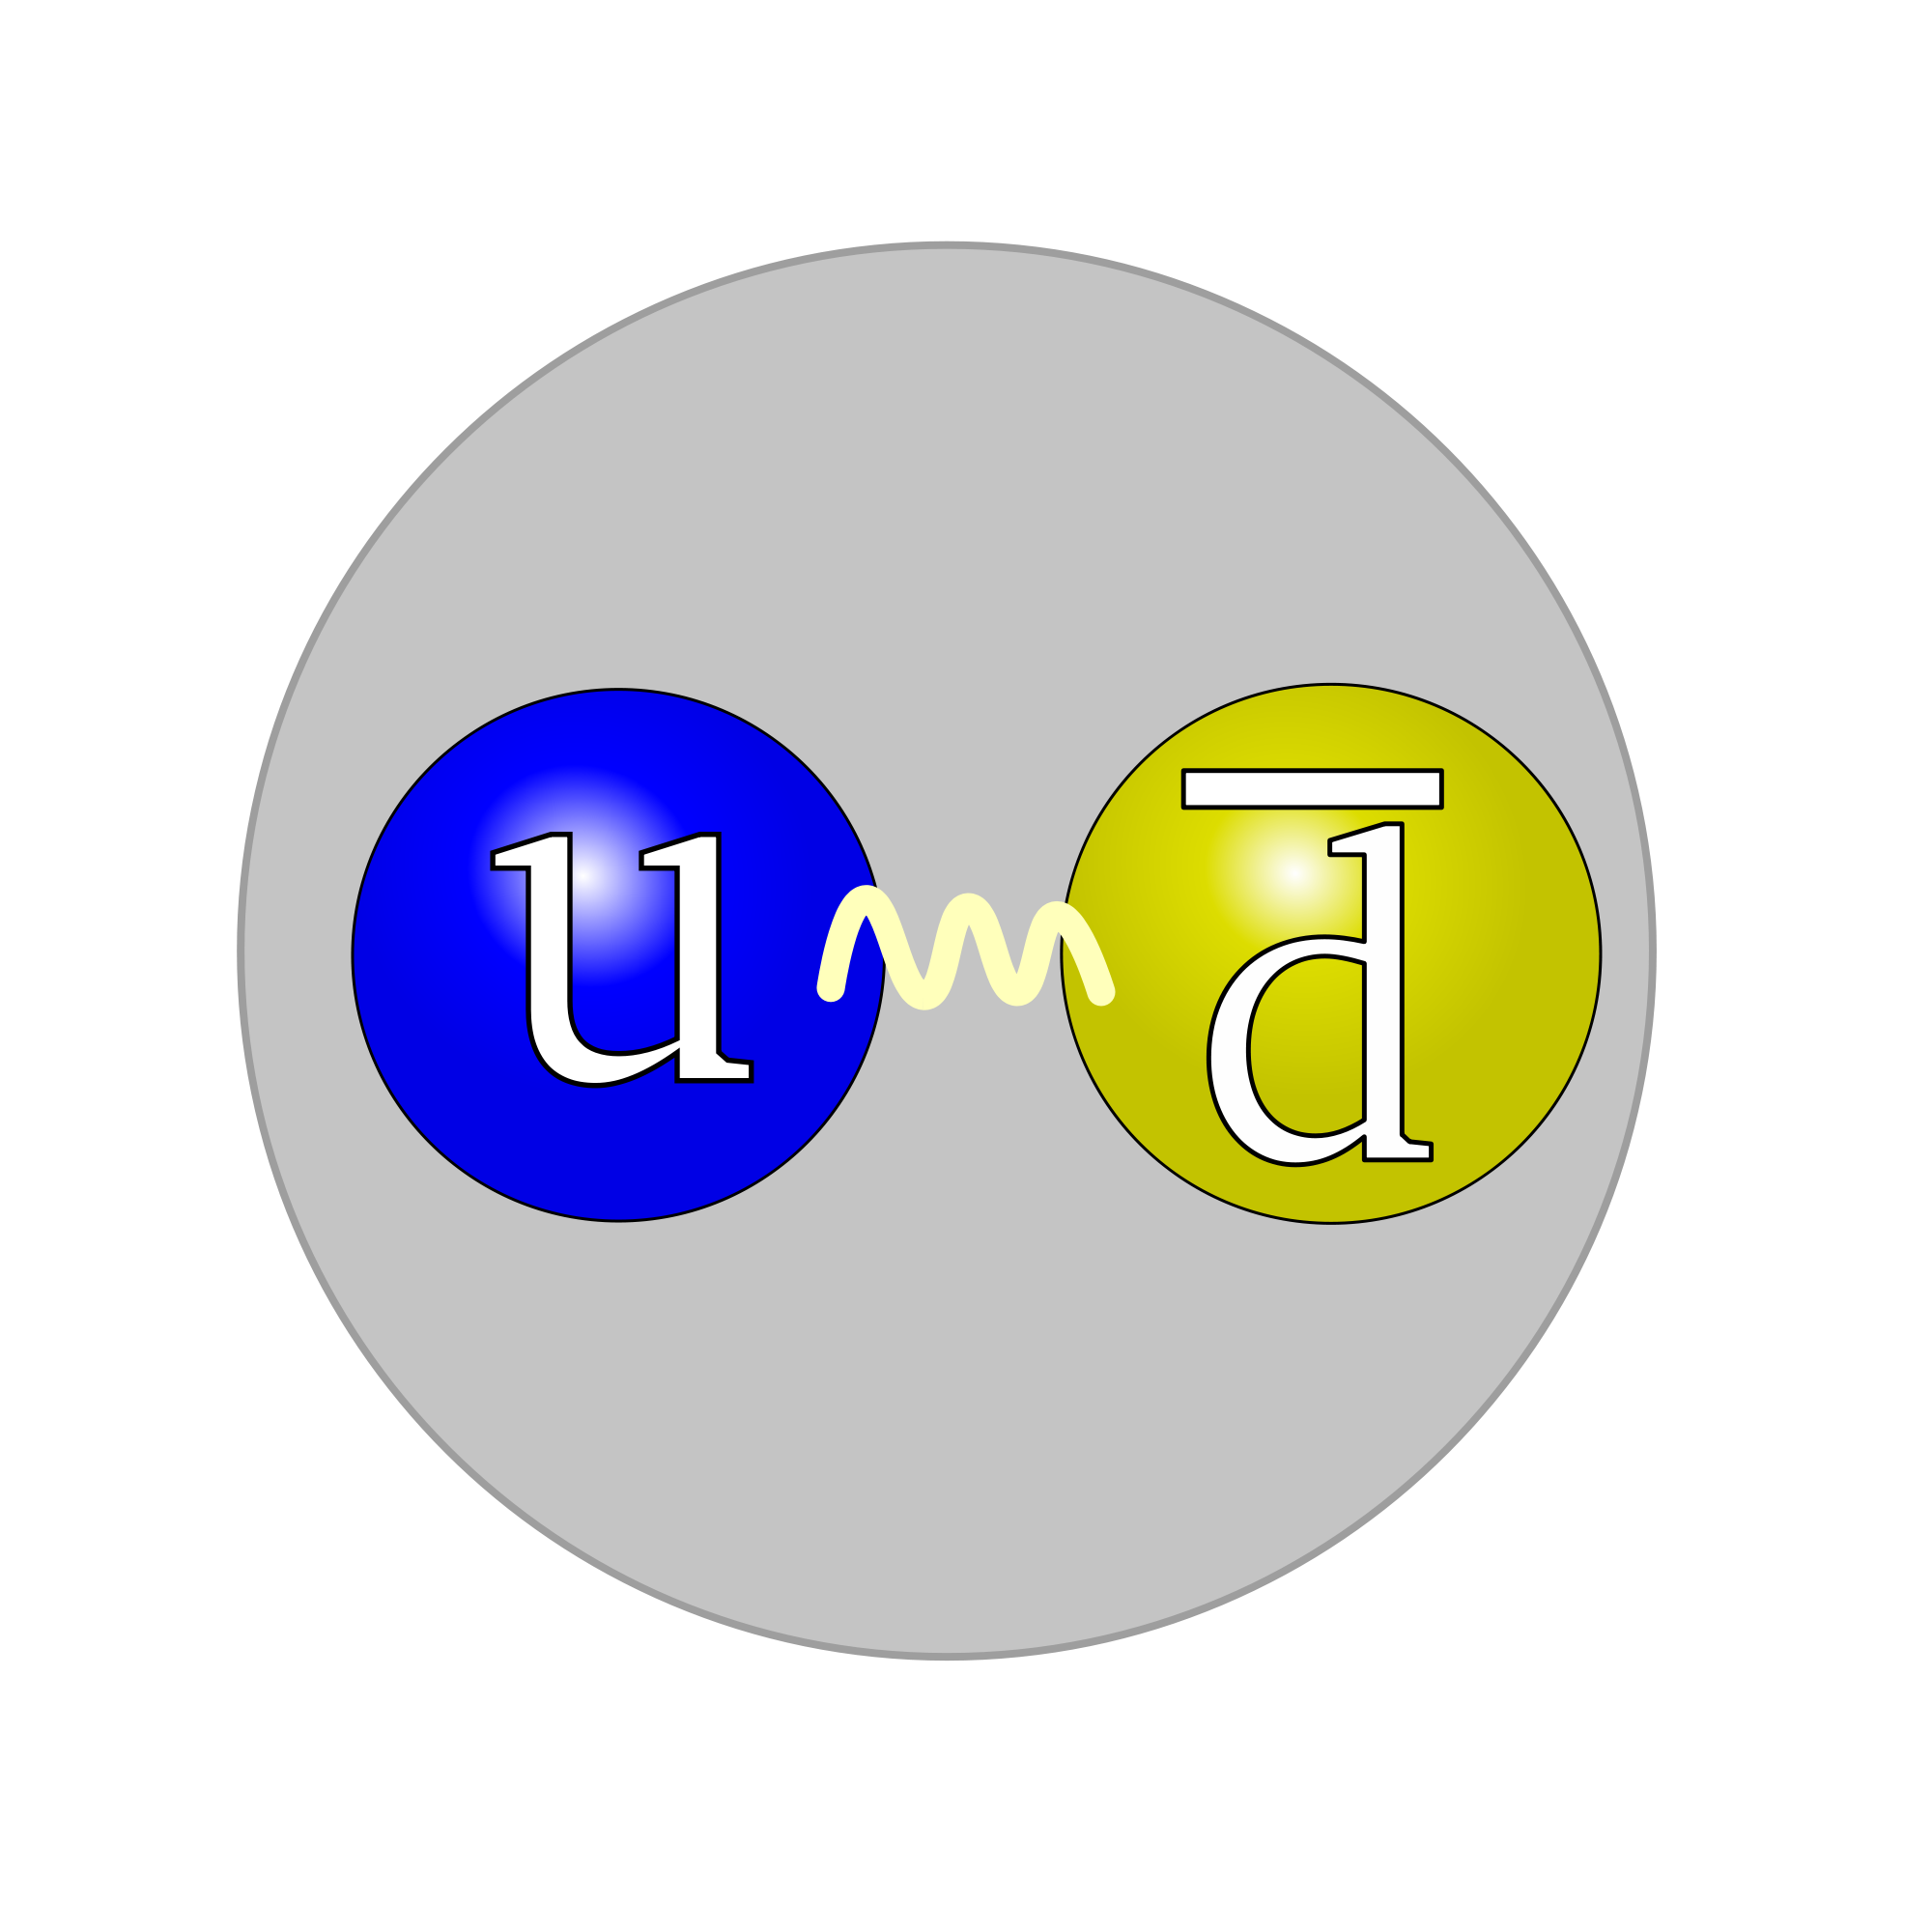
\includegraphics[width=0.5\textwidth]{ImgChap1/Meson2}
	\caption{Test results of the different reflective materials. Rate at different levels of the discriminator.}
	\label{ReflTestResults}
\end{figure}

Taking into account the literature and tests carried out the tiles. Titanium dioxide paint was selected as the material which best satisfied the demands required of the material, with a high reflective index, consistent results and ease of application. The PTFE was both thin and highly reflective, but the difficulty in wrapping the tiles with their projecting fibres in a consistent manner, was a major downside to this choice of reflector. A combination approach applying PTFE to most of the tile and covering the awkward areas with titanium dioxide paint was also considered, but discarded as the performance of PTFE was comparable to the paint in the tests carried out.

Aluminium foil was used 
Specular and diffuse reflectors.


Transition between materials important. Light loss at boundary. Change of refractive index.
Reflective paint, alumised mylar, aluminised sputtering, tyvek, ptfe etc.
Discussion of diffuse reflectors vs specular reflectors.
Issues with wrapping of the tiles.
Mirroring the ends of the fibres.
Very important to achieve consistency accross the tiles.
High reflectivity essential to achieve a large photon output after multiple reflections.
High reflectivity also essential to maintain optical isolation between elements and minimise crosstalk.
Thickness of material a major concern as this limits the acceptance of the detector. Want to be as thin as possible.
Cost also a consideration, sputtering a large number of tiles would be very expensive.
Variation of results of studies in the literature. Partly dependent on the test conditions favouring one configuration over another. Essential to carry out bespoke studies for the detector system, to ensure the right option was selected.
\cite{janecek2012reflectivity}
\cite{janecek2008optical}
\cite{weidner1981reflection}
\textbf{Need to find the other references that were used to make this decision}
\subsubsection{Mirroring of the end of the fibres}

Wavelength shifting fibres operate by absorbing a photon before remitting it in a new frequency range. For this photon to be captured and transmitted down the length of the fibre, it needs to be produced in a narrow emission of of a few degrees. The vector of re-emission is not dependent on the angle of incidence of the original photon. As a consequence, mirroring the scintillor end of the fibre, allows the angle of acceptance for capturing the photon within the fibre to potentially be almost doubled. This comes at the cost of blocking any photons that may have entered the fibre through the end of the fibre, but in a fibre of any significant length the benefits outweigh the downsides.

The ideal reflector for this purpose shares many of the same characteristics as for the scintillators, but it also has the conform to the limitations of attaching to the end of a fibre at the end of a narrow channel.  To be effective the reflector needs to cover the full area of the fibre, particularly as the multi-layered design of the fibres results in the majority of light being transported in a narrow region near the edge of the fibre. However if it is fractionally larger than the fibre it will either not fit, damage or be damaged when placed into the channel. In most examples in the literature such as the study done by Joram \cite{joram2014mirroring}. The mirrored fibres were placed in flat channels which pass all the way across the scintillator where there was easy access to the ends of the fibres. However the design of the hodoscope restricts this access and tests using an idealise reflector such as thin disks of aluminised mylar were inconsistent in tests. After these the titanium dioxide paint used as the reflector on the scintillators was considered along with aluminium sputter depsoition, which would deposit a thin layer of aluminium directly onto the fibres. However the latter option was ruled out on cost effectiveness after tests using the reflective paint proved highly effective and consistent. 

\cite{joram2014mirroring}
\subsection{Optical Connections and transport}

Transitions between transport materials are a critical element of efficient photon transport. A simplistic overview of each photons journey in a channel would start with production in the scintillating tiles, transport through the optical fibres before arrival at the the SiPMs. However there are transition points between the tile and WLS fibres, WLS fibres and clear fibres, and from the clear fibres to the SiPMs. Along with the less obvious transitions between layers in the fibres.  

Transparent materials with similar refractive indices minimise the amount of photons lost at the boundary between materials. How much of this is due to internal reflections? Consider transition radiation at boundaries, cherenkov radiation and any other effects that may contribute to the loss in signal strength.

Discussion on ideal optical properties, however these must maintain their quality under radiation and age. Affects of any annealing. Consistent properties essential for proper calibration of the equipment over time.

Possible discussion on fusion splicing could go here instead of in the optical transport section. Or could combine the two together.

Optical glues and their properties. Transmission ideal, similar refractive index, hermetic and uniform response. Radiation hard. Tested under similar conditions. Will not damage the fragile materials around it.

Comparison to an air connection, why use glue if an air connection would do? Not possible in this case due to the tension in the fibres and orientation of the hodoscope. The fibres would simply fall out of the holes! Ensuring the fibres fill the entire length of the channel, extremely important to maximise the light output of the tiles and also maintain uniform response of all the channels.

Air connection used for the SiPMs but the fibres are fixed into the connectors. Gluing the fibres to the SiPMs would make mainanence impossible. 

Glues, fibre joins, fusion spicing, fibre to SiPM.
\subsection{Glues}
\cite{kobayashi1991transmittance}
\cite{kirn1999absorption}
\cite{clements2006selection}
\cite{montecchi2001study}
\cite{cohen2003optical}
\cite{cohen2001optical}
\cite{va2014optical}

\subsection{Forward Tagger Flasher Flasher}

Used for measuring the change sensitivity of the fibres and tiles over time, by using a driver of constant manitude to radiate the system and measure the level of output throughout the lifetime of the detector.

\section{Effect of radiation on different components}
Critically the effect on the scintillator tiles and the light transport components along with the SiPM. Mostly just the components that are part of the lollypop will be under significant levls of radiation.
Discuss the annealing process for the scintillator and fibres. How this offsets the damage that the radiation will do.
The detector is shielded from much of the intense radiation by the moeller cone. 

\cite{bross1990radiation}
\cite{barsuk2000radiation}
\cite{protopopov1993radiation}
\section{Testing}
While designing each element of the detector.
Sample testing on arrival.
During construction.
Beam tests.
Photon Output.
Bend radius.
Calibration using different ratioactive sources, or cosmic rays. Problems and benefits of each method of testing.
Ideally testing the equipment with a beam similar in nature to the processes that will be carried out at JLAB. However there is limited availability of beam time and compromises are needed between rate and precision. Source vs cosmic normally.
Construction stress tests.
\section{Beamtime}
Frascati tests.
\section{Contruction}
Everything tested and built in a very low UV enviroment to protect the fibres and tiles.
Air was filtered.
Air was cooled to keep and standard temperature for testing.
Lab coats, gloves etc.


\subsection{Component arrangement and Numbering systems}
How the tiles were arranged.
Measuring the sizes of each tile to optimise the arrangement through the detector and minimise any gaps, maximising the effective coverage and this acceptance of the detector system. Focusing on the areas of highest flux where detector acceptance is most critical to be near perfect.
Arranging the position and orientation of the tiles to maximise the efficiency of the fibre packing to minimise the vertical space taken up by the fibres and reducing and pressure load on the fibres. Identifying any critical areas of strain and how to deal with these pressure points.
Arranging the fibres to fit into bundles, then how they would path through the detector, fit into the delta wing and transition through CLAS to reach the electronics.
Arranging the bundles on the way to the electronics. The bundles must fit through tight space requirements, where maximising packing efficiency is critical. The fibres must be kept protected from damage and sealed from any outside sources of light or crosstalk.
\subsection{Numbering system for the elements of the detector system}
Sections of the detector.
Fibre bundles.
\subsection{Gluing} 
Different types of glue. Studies on their transmitivity properties, effect of radiation damage, pot life (too fast and too much heat that will damage the fibres and tiles).
Precise scales and pippetes used to ensure quality and consistency of the mix. Mixed thoroughly and then put under vacuum to remove any air bubbles.
Different glues used for holding the fibres in place in the delta wings and affixing the fibres into the tiles.
\section{Detector Longevity}
Expected effect of running on the detector.
Radiation damage.
Electronic issues.

\section{Commissioning}
Calibrating, optimising, fixing any problems and resolving any unforeseen issues.
\section{Future development}
Upgrades to the electronics crate to provide fan cooling to the SiPM boards. Allowing them to be running at a higher operating voltage 